\documentclass[13pt,a4paper,final]{article}

\usepackage[12pt]{extsizes}
\usepackage[T2A]{fontenc}
\usepackage[utf8]{inputenc}
\usepackage[russian]{babel}
\usepackage{amsmath}
\usepackage{amssymb}
\usepackage{tikz}
\usepackage{wrapfig}
\usepackage{ragged2e}
\usepackage{rotating}
\usepackage{float}
\usepackage{xltabular}
\usepackage{hyperref}
\usepackage[left=23mm, top=20mm, right=20mm, bottom=20mm, footskip=10mm]{geometry}
\usepackage{setspace}
\usepackage{moreverb}
\usepackage{indentfirst}
\renewcommand\verbatimtabsize{4\relax}
\renewcommand\listingoffset{0.2em}
\renewcommand{\arraystretch}{1.4}
\usepackage[font=small, singlelinecheck=false, justification=raggedleft, format=plain, labelsep=period]{caption}
\usepackage{listings}
\usepackage{xcolor}
\usepackage{alltt}
\usepackage{enumitem}
\usepackage{pdflscape}
\usepackage{pdfpages}
\DeclareMathOperator\arcth{arcth}
\DeclareMathOperator\arccth{arccth}
\pagestyle{plain}
\usepackage{array}
\usepackage{graphicx}
\usepackage{longtable}
\usepackage{colortbl}
\usepackage{listingsutf8}
\definecolor{codegreen}{rgb}{0,0.6,0}
\definecolor{codegray}{rgb}{0.5,0.5,0.5}
\definecolor{codepurple}{rgb}{0.58,0,0.82}
\definecolor{backcolour}{rgb}{0.95,0.95,0.92}
\hypersetup{colorlinks, allcolors=[RGB]{000 000 000}}
\lstdefinestyle{mystyle}{
	backgroundcolor=\color{backcolour},
	commentstyle=\color{codegreen},
	keywordstyle=\color{magenta},
	numberstyle=\tiny\color{codegray},
	stringstyle=\color{codepurple},
	basicstyle=\ttfamily\footnotesize,
	breakatwhitespace=false,
	breaklines=true,
	captionpos=t,
	keepspaces=true,
	numbers=left,
	numbersep=5pt,
	showspaces=false,
	showstringspaces=false,
	showtabs=false,
	tabsize=2
}
\setlist[enumerate,itemize]{leftmargin=1.7cm}
\lstset{style=mystyle}
\lstset{extendedchars=\true}
\lstset{escapeinside={(*@}{@*)}}
\captionsetup[figure]{justification=centering}
\addto\captionsrussian{\def\refname{Список использованной литературы}}

\begin{document}
	
	\begin{center}
		\normalsize{МИНИСТЕРСТВО НАУКИ И ВЫСШЕГО ОБРАЗОВАНИЯ РОССИЙСКОЙ ФЕДЕРАЦИИ\\
			федеральное государственное автономное образовательное учреждение высшего образования «Санкт-Петербургский политехнический университет Петра Великого»\\[10pt]}
		\normalsize{Институт компьютерных наук и кибербезопасности}\\[10pt]
		\normalsize{Высшая школа технологий искусственного интеллекта}\\[10pt]
		\normalsize{Направление: 02.03.01 <<Математика и компьютерные науки>>}\\
		
		\hfill \break
		\hfill \break
		\hfill \break
		\hfill \break
		\hfill \break
		\hfill \break
		\normalsize{}\\
		\large{Отчёт по курсовой работе}\\
		\normalsize{по дисциплине <<Защита информации>>}\\
		\large{<<Разработка программного обеспечения межсетевого экрана>>}\\
		\hfill \break
		\hfill \break
		\hfill \break
		\hfill \break
		\hfill \break
		\hfill \break
	\end{center}
	
	\hspace{-0.8cm}Группа \hspace{\fill}  \hspace{3cm}\hspace{5pt} 5130201/30101\\\\
	
	\hspace{-0.8cm}Преподаватель
	
	\hfill\hspace{80pt} \rule[0.25ex]{3cm}{0.4pt} \hspace{5pt} Силиненко А. В. \hspace{-6.8cm}
	\hfill \break
	\hfill \break
	\hfill \break
	
	\hfill \break
	\hfill \break
	\hfill \break
	\hfill \break
	\hfill \break
	\hfill \break
	\begin{center} \small{Санкт-Петербург}
	\end{center}
	\begin{center} \small{2026}
	\end{center}
	\thispagestyle{empty}
	
	\newpage
	\section*{Список исполнителей}
	\textbf{Тимлид} — Радионова Полина Викторовна
	
	\textbf{Аналитика}:
	\begin{enumerate}
		\item Васюк Марина Витальевна
		\item Лаишевкина Анна Максимовна
		\item Мелещенко Софья Игоревна
		\item Толчина Алёна Сергеевна
	\end{enumerate}
	
	\textbf{ПС-1 Фильтрация}:
	\begin{enumerate}
		\item Егоров Святослав Андреевич
		\item Ерошкин Кирилл Алексеевич
		\item Чиботарь Андрей Иванович
		\item Шишмаков Владимир Олегович
		\item Янковский Эрик Алексеевич
	\end{enumerate}
	
	\textbf{ПС-2 Регистрация}:
	\begin{enumerate}
		\item Гордиенко Юлия Артемовна
		\item Уэссу Дональде Памела Махуна
		\item Черепанова Надежда Сергеевна
	\end{enumerate}
	
	\textbf{ПС-3 CLI} и \textbf{ПС-4 WEB}:
	\begin{enumerate}
		\item Иванова Варвара Антоновна
		\item Мартыненко Анна Павловна
		\item Назмеева Алина Рифовна
		\item Попов Илья Александрович
		\item Саитгареев Ратмир Ильдарович
	\end{enumerate}
	
	
	\textbf{ПС-5 Авторизация} и \textbf{ПС-6 Целостность}:
	\begin{enumerate}
		\item Волнухина Виктория Денисовна
		\item Карцев Сергей Михайлович
		\item Митяев Олег Игоревич
		\item Цыбукова Софья Дмитриевна
	\end{enumerate}
	
	
	\newpage
	\tableofcontents
	\newpage
	\section{Спецификация требований к ПО МЭ}
	\subsection{Общие сведения}
	\subsubsection{Назначение}
	Программное обеспечение межсетевого экрана (ПО МЭ) предназначено для фильтрации сетевого трафика в соответствии с политикой доступа. 
	\subsubsection{Среда функционирования}
	\begin{itemize}
		\item ОС: Linux, дистрибутив Debian 12, архитектура x86\_64.
		\item Сетевые порты: от 1 до 6 портов Ethernet 1 Гб/с; число используемых портов определяется конфигурацией.
		\item Поддерживаемые протоколы: Ethernet, IPv4, TCP, UDP, ICMPv4.  Кадры ARP и кадры других протоколов Ethernet обрабатываются по правилам с полем \texttt{eth-proto} (FR-11).
	\end{itemize}
	
	\subsubsection{Режим работы}
	МЭ работает в прозрачном режиме (L2): принимает кадры на всех интерфейсах и передаёт разрешённые кадры на выходные интерфейсы, указанные в правиле (обоснование — п. 2.6). IP-адреса интерфейсов и системные маршруты используются только для трафика самого МЭ (управление по SSH и HTTPS) и не влияют на пересылку транзитного трафика.
	
	\subsubsection{Ограничение и допущения}
	\begin{itemize}
		\item Один экземпляр ПО МЭ управляет одним устройством; кластеризация и отказоустойчивость не рассматриваются.
		\item Пропускная способность 1 Гб/с на порт — целевое значение; измеряется для правил без флага регистрации (раздел 1.4).
		\item Контроль состояний выполняется только для TCP, UDP и ICMP Echo (ping). Прочие сообщения ICMP, в том числе сообщения об ошибках, обрабатываются как первые пакеты по политике доступа.
		\item Контроль состояний TCP выполняется по флагам и направлению пакетов; номера последовательности не проверяются.
		\item Восстановление повреждённых контролируемых файлов~--- штатная операция: администратор выполняет её командой \texttt{integrity restore} в CLI (или в web-интерфейсе) из резервной копии (FR-49). Резервные копии и эталонные контрольные суммы формируются до установки ПО (FR-50).
	\end{itemize}
	
	\subsubsection{Термины и сокращения}
	\begin{xltabular}{\textwidth}{|X|X|}
		\caption{Термины и сокращения} \\
		\hline
		\textbf{Термин} & \textbf{Определение} \\
		\hline
		\endfirsthead
		\hline
		\multicolumn{2}{|l|}{\small\itshape Продолжение таблицы \thetable} \\
		\hline
		\textbf{Термин} & \textbf{Определение} \\
		\hline
		\endhead
		\hline
		\multicolumn{2}{r|}{\small\itshape Продолжение на следующей странице...} \\
		\endfoot
		\hline
		\endlastfoot
		МЭ / ПО МЭ & Межсетевой экран / программное обеспечение межсетевого экрана \\
		\hline
		ПС & Подсистема – отдельный процесс ПО МЭ \\
		\hline
		Политика доступа & Упорядоченный набор правил фильтрации, нумеруемых целыми числами \\
		\hline
		Соединение & Логически связанные пакеты TCP, UDP или ICMP Echo между двумя узлами с общим ключом состояния \\
		\hline
		Таблица состояний & Список активных соединений, по которым принимаются решения для пакетов, кроме первого \\
		\hline
		Журнал событий & Хранилище записей о событиях управления и работы МЭ \\
		\hline
		Журнал трафика & Хранилище записей об обработанных пакетах \\
		\hline
		Сеанс администратора & Период работы администратора от входа до выхода или сброса \\
		\hline
		Контролируемые файлы & Исполняемые и конфигурационные файлы МЭ, целостность которых проверяется \\
		\hline
		Режим аварийной поддержки & Режим без обработки трафика, в котором администратор восстанавливает целостность файлов \\
		\hline
		ПМИ & Программа и методика испытаний (ГОСТ 19.301-79) \\
		\hline
		FR-xx & Функциональное требование задания 3 \\
		\hline
		Вне контекста соединения & Пакет, не соответствующий ни одной записи таблицы состояний и не являющийся допустимым первым пакетом нового соединения \\
		\hline
	\end{xltabular}
	
	\subsection{Внешние интерфейсы и данные}
	\subsubsection{Входные и выходные данные}
	Входные данные:
	\begin{itemize}
		\item сетевой трафик — кадры Ethernet с пакетами IPv4 (TCP, UDP, ICMPv4), поступающие на интерфейсы МЭ;
		\item команды администратора в командном интерфейсе (локально с консоли, удалённо по SSH, п. 2.7) и в web-интерфейсе (по HTTPS, п. 2.8);
		\item файлы конфигурации, политики доступа, учётных записей и эталонных контрольных сумм (п. 1.2.6).
	\end{itemize}
	
	Выходные данные:
	\begin{itemize}
		\item переданные на выходные интерфейсы или удалённые пакеты;
		\item записи журнала событий и журнала пакетов (FR-25, FR-26);
		\item ответы командного и web-интерфейсов: результаты команд и сообщения (п. 1.2.5).
	\end{itemize}
	
	\subsubsection{Правило фильтрации}
	\begin{xltabular}{\textwidth}{|p{3.5cm}|p{3cm}|p{5cm}|p{3.5cm}|}
		\caption{Поля правила фильтрации} \\
		\hline
		\textbf{Поле} & \textbf{Аргумент CLI} & \textbf{Допустимые значения} & \textbf{По умолчанию} \\
		\hline
		\endfirsthead
		\hline
		\multicolumn{4}{|l|}{\small\itshape Продолжение таблицы \thetable} \\
		\hline
		\textbf{Поле} & \textbf{Аргумент CLI} & \textbf{Допустимые значения} & \textbf{По умолчанию} \\
		\hline
		\endhead
		\hline
		\multicolumn{4}{r|}{\small\itshape Продолжение на следующей странице...} \\
		\endfoot
		\hline
		\endlastfoot
		Номер правила & N (позиционный) & Целое число 1–65535, уникальное & {обязателен} \\
		\hline
		Входной интерфейс & in & Имя интерфейса из конфигурации или any & any \\
		\hline
		MAC-адрес источника / приёмника & smac, dmac & XX:XX:XX:XX:XX:XX или any & any \\
		\hline
		IPv4-адрес источника / приёмника & src, dst & Адрес, адрес с маской (CIDR, маска 0–32), диапазон или any & any \\
		\hline
		Протокол IP & proto & tcp, udp, icmp, номер 0–255 или any & any \\
		\hline
		Другие протоколы Ethernet & eth-proto & arp, other, any & any \\
		\hline
		Порт источника / приёмника & sport, dport & 1–65535 или диапазон; только при proto=tcp или udp & any \\
		\hline
		Тип и код ICMPv4 & icmp-type, icmp-code & 0–255; только при proto=icmp & any \\
		\hline
		Действие & action & accept (передать), goto (перейти к правилу), drop (удалить) & {обязателен} \\
		\hline
		Выходные интерфейсы & out & Список интерфейсов; обязателен при action=accept; не включает входной интерфейс & — \\
		\hline
		Переход к правилу & to & Номер существующего правила, больший номера текущего; обязателен при action=goto & — \\
		\hline
		Контроль состояния & state & on (контролировать) / off; действует только при action=accept & off \\
		\hline
		Активность & active & yes / no & yes \\
		\hline
		Регистрация & log & yes (регистрировать) / no & no \\
		\hline
		Комментарий & comment & Строка до 255 символов & пусто \\
		\hline
	\end{xltabular}
	
	В web-форме правила поля, зависящие от протокола и действия (порты, тип и код ICMP, выходные интерфейсы, переход, контроль состояния), показываются только при соответствующем значении протокола или действия; ошибки проверки выводятся рядом с полем.
	\subsubsection{Параметры конфигурации}
	\begin{xltabular}{\textwidth}{|X|X|X|}
		\caption{Параметры конфигурации} \\
		\hline
		\textbf{Параметр} & \textbf{По умолчанию} & \textbf{Допустимые значения} \\
		\hline
		\endfirsthead
		\hline
		\multicolumn{3}{|l|}{\small\itshape Продолжение таблицы \thetable} \\
		\hline
		\textbf{Параметр} & \textbf{По умолчанию} & \textbf{Допустимые значения} \\
		\hline
		\endhead
		\hline
		\multicolumn{3}{r|}{\small\itshape Продолжение на следующей странице...} \\
		\endfoot
		\hline
		\endlastfoot
		Таймауты TCP & Синхронизация (SYN) — 5 с; Установлено (ESTABLISHED) — 3600 с; Финализация (FIN/TIME\_WAIT) — 30 с & 1–86400 с \\
		\hline
		Таймауты UDP & 15 с без ответа; 60 с после ответа & 1–86400 с \\
		\hline
		Таймаут ICMP & 5 с & 1–86400 с \\
		\hline
		Размер таблицы состояний & 65536 записей & 1024–1048576 \\
		\hline
		Контроль состояний & Включён & вкл / выкл \\
		\hline
		Пересылка ARP (FR-11) & Выключена & вкл / выкл \\
		\hline
		Политика ARP по умолчанию & Правило \texttt{eth-proto=arp}, \texttt{action=accept}, \texttt{out}=все интерфейсы кроме входного & — \\
		\hline
		Управляющие интерфейсы & Один интерфейс, задаётся при установке & список интерфейсов \\
		\hline
		Порты управления & SSH — 22, HTTPS — 8443 & 1–65535 \\
		\hline
		Период проверки целостности & 60 с & 10–3600 с \\
		\hline
		Блокировка входа & 5 неудачных попыток подряд, блокировка на 60 с & — \\
		\hline
		Завершение сеанса при бездействии & 15 минут & — \\
		\hline
		Предел журнала пакетов / событий & 100 МБ / 50 МБ & 1–1024 МБ \\
		\hline
		Размер страницы вывода & CLI — 20 записей, web — 50 записей & — \\
		\hline
	\end{xltabular}
	
	Конфигурация по умолчанию также содержит пустую политику доступа (все пакеты IPv4 удаляются, FR-08), настройку для пересылки ARP (\texttt{eth-proto=arp}, \texttt{action=accept}) и предустановленного администратора (FR-33).
	\subsubsection{Коды событий}
	\begin{xltabular}{\textwidth}{|c|X|}
		\caption{Коды событий журнала событий} \\
		\hline
		\textbf{Код} & \textbf{Событие} \\
		\hline
		\endfirsthead
		\hline
		\multicolumn{2}{|l|}{\small\itshape Продолжение таблицы \thetable} \\
		\hline
		\textbf{Код} & \textbf{Событие} \\
		\hline
		\endhead
		\hline
		\multicolumn{2}{r|}{\small\itshape Продолжение на следующей странице...} \\
		\endfoot
		\hline
		\endlastfoot
		E01 & Вход администратора \\
		\hline
		E02 & Выход администратора \\
		\hline
		E03 & Неуспешная попытка входа \\
		\hline
		E04 & Понижение прав администратора до «только чтение» \\
		\hline
		E05 & Сброс сеанса администратора другим администратором \\
		\hline
		E06 & Блокировка входа после 5 неудачных попыток \\
		\hline
		E07 & Завершение сеанса по бездействию или из-за удаления учётной записи \\
		\hline
		E10 & Включение МЭ \\
		\hline
		E11 & Выключение МЭ \\
		\hline
		E12 & Запуск подсистемы \\
		\hline
		E13 & Остановка или перезагрузка подсистемы \\
		\hline
		E14 & Включение механизма контроля состояний \\
		\hline
		E15 & Отключение механизма контроля состояний \\
		\hline
		E20 & Добавление правила политики доступа \\
		\hline
		E21 & Изменение правила политики доступа \\
		\hline
		E22 & Удаление правила политики доступа \\
		\hline
		E30 & Изменение конфигурационного параметра \\
		\hline
		E31 & Сохранение, применение или сброс конфигурации \\
		\hline
		E32 & Изменение учётной записи \\
		\hline
		E33 & Изменение параметров интерфейса, маршрутов, даты и времени \\
		\hline
		E34 & Очистка журнала пакетов \\
		\hline
		E35 & Удаление записей из таблицы состояний \\
		\hline
		E36 & Переполнение журнала пакетов, замена старых записей \\
		\hline
		E37 & Переполнение журнала событий, удаление старых записей \\
		\hline
		E40 & Нарушение целостности контролируемых файлов \\
		\hline
		E41 & Восстановление целостности, возобновление обработки трафика \\
		\hline
		E42 & Проверка целостности по запросу администратора (результат) \\
		\hline
		E43 & Неуспешное завершение изменяющей операции администратором (с указанием причины) \\
		\hline
		E50 & Отказ в доступе: недостаточно прав для выполнения команды (с указанием команды) \\
		\hline
	\end{xltabular}
	
	\subsubsection{Сообщения и ошибки}
	При любой ошибке операция не выполняется и состояние МЭ не изменяется. Необработанные исключения не завершают процесс интерфейса.
	\begin{xltabular}{\textwidth}{|c|X|X|}
		\caption{Сообщения} \\
		\hline
		\textbf{Код} & \textbf{Сообщение} & \textbf{Когда выводится} \\
		\hline
		\endfirsthead
		\hline
		\multicolumn{3}{|l|}{\small\itshape Продолжение таблицы \thetable} \\
		\hline
		\textbf{Код} & \textbf{Сообщение} & \textbf{Когда выводится} \\
		\hline
		\endhead
		\hline
		\multicolumn{3}{r|}{\small\itshape Продолжение на следующей странице...} \\
		\endfoot
		\hline
		\endlastfoot
		M01 & Введите идентификатор: / Введите пароль: & Приглашение при входе \\
		\hline
		M02 & Ошибка: неверный идентификатор или пароль & {Неуспешная аутентификация (FR-30)} \\
		\hline
		M03 & Ошибка: недостаточно прав. Режим «только чтение» & Изменяющая команда от администратора с правами «только чтение» (FR-32) \\
		\hline
		M04 & Внимание: права понижены до «только чтение», так как активен другой администратор с правами {«чтение/запись»} & Вход второго администратора с правами «чтение/запись» {(FR-34)} \\
		\hline
		M05 & Ошибка: удалять предустановленного администратора или менять его роль запрещено & FR-33 \\
		\hline
		M06 & Ошибка: неверное значение поля «тип поля». \newline {Допустимые значения: диапазон} & Нарушение формата или диапазона параметра \\
		\hline
		M07 & Ошибка: правило с номером N уже существует / не найдено & Конфликт или отсутствие номера правила \\
		\hline
		M08 & Ошибка: нарушена целостность файлов. Трафик заблокирован. \newline {Режим аварийной поддержки} & Нарушение целостности (FR-48) \\
		\hline
		M09 & Операция выполнена & Успешное выполнение изменяющей команды \\
		\hline
		M10 & Ошибка: недопустимая операция в режиме аварийной поддержки & FR-49 \\
		\hline
		M11 & Ошибка: на правило {ссылается} правило N (переход). Удаление запрещено & Удаление правила, на которое есть переход {(FR-13)} \\
		\hline
		M12 & Ошибка: вход временно заблокирован. Повторите через 60 с & FR-31 \\
		\hline
		M13 & Записи не найдены & Пустая выборка \\
		\hline
		M14 & Ошибка: неизвестная команда. Введите help & Команда не распознана CLI \\
		\hline
		M15 & Сеанс завершён: «причина» & Завершение сеанса по бездействию, сбросу или удалению учётной записи (FR-36) \\
		\hline
		M16 & Ошибка: подсистема «имя» не отвечает. Операция не выполнена & Нет ответа подсистемы после повторных запросов (таймаут обмена) \\
		\hline
	\end{xltabular}
	\subsubsection{Хранимые данные}
	\begin{xltabular}{\textwidth}{|X|X|X|}
		\caption{Данные и их хранение} \\
		\hline
		\textbf{Данные} & \textbf{Состав} & \textbf{Хранение} \\
		\hline
		\endfirsthead
		\hline
		\multicolumn{3}{|l|}{\small\itshape Продолжение таблицы \thetable} \\
		\hline
		\textbf{Данные} & \textbf{Состав} & \textbf{Хранение} \\
		\hline
		\endhead
		\hline
		\multicolumn{3}{r|}{\small\itshape Продолжение на следующей странице...} \\
		\endfoot
		\hline
		\endlastfoot
		Политика доступа & Правила с полями из таблицы 2 & {файл JSON} \\
		\hline
		Конфигурация & Параметры из таблицы 3, параметры интерфейсов и системы; текущая, сохранённая, по умолчанию & {файлы JSON} \\
		\hline
		Учётные записи & Идентификатор, хэш пароля с солью, роль, признак предустановленной учётной записи & {файл учётных записей} \\
		\hline
		Активные сеансы & Идентификатор, роль, интерфейс (CLI/web), IP-адрес, время входа и последнего действия & В памяти и служебный файл \\
		\hline
		{Таблица состояний} & Ключ соединения (IP-адреса и порты источника и приёмника), протокол, состояние, таймер, счётчики, входной и выходные интерфейсы, номер правила & {В памяти процесса ПС-1 (подсистема фильтрации)} \\
		\hline
		Журнал событий & Поля по FR-25 & {База данных SQLite} \\
		\hline
		Журнал пакетов & Поля по FR-26 & Двоичный кольцевой файл на диске (записи фиксированной длины); запись блоками через буфер в памяти \\
		\hline
		Эталонные контрольные суммы & Путь файла и хэш SHA-256 & Файл, защищённый HMAC (FR-47), {владелец~--- пользователь ОС fw-integrityd (ПС-6)} \\
		\hline
		{Резервные копии} & Копии контролируемых файлов & Каталог, {владелец~--- пользователь ОС fw-integrityd (ПС-6)} \\
		\hline
	\end{xltabular}
	
	Журналы доступны администратору только для чтения; изменить их можно только очисткой журнала пакетов (FR-40).
	
	Описания командного и web-интерфейсов администратора вынесены в раздел 2 (п. 2.7, 2.8).
	
	\subsection{Функциональные требования}
	В скобках указан пункт задания (ТЗ), из которого следует требование. Требования без ссылки на ТЗ уточняют поведение МЭ.
	
	\subsubsection{Ввод данных и запуск}
	
	\textbf{FR-01 (ТЗ 1.2, 2.1)}. МЭ должен принимать кадры Ethernet на всех включённых интерфейсах (от 1 до 6) и обрабатывать весь поступающий трафик.
	
	\textbf{FR-02 (ТЗ 4.1, 5.1, 5.2)}. Командный интерфейс должен быть доступен с консоли МЭ и удалённо по SSH. При удалённом управлении SSH-соединение устанавливается под выделённой учётной записью ОС, для которой принудительно запускается CLI МЭ (ForceCommand); вход в ОС не даёт доступа к функциям управления без аутентификации в МЭ. IP-адрес администратора определяется по параметрам SSH-соединения.
	
	\textbf{FR-03 (ТЗ 5.1, 5.2)}. Web-интерфейс должен принимать запросы по HTTPS с удалённого компьютера через управляющий интерфейс и локально по адресу 127.0.0.1.
	
	\textbf{FR-04}. При запуске ПО МЭ должно считывать конфигурацию и политику доступа. Учётные записи хранятся в файле и при запуске не считываются: ПС-5 обращается к файлу по мере необходимости~--- при входе администратора и при операциях с учётными записями. Если сохранённых файлов {конфигурации и политики} нет (первый запуск), загружаются значения по умолчанию и регистрируется E31. Если хэш хотя бы одного контролируемого файла не совпадает с эталонным значением или нарушен HMAC файла эталонов, МЭ переходит в режим аварийной поддержки (FR-48). {ПС-1 стартует в заблокированном состоянии (\texttt{emergency\_mode=1}); загрузка политики доступа выполняется только после успешной проверки целостности ПС-6.}
	\subsubsection{Фильтрация трафика (ТЗ 2.1–2.3)}
	
	\textbf{FR-05 (ТЗ 2.2)}. МЭ должен проверять каждый пакет на соответствие правилам политики доступа по критериям: входной интерфейс; MAC-адреса источника и приёмника; IPv4-адреса источника и приёмника; протокол, инкапсулированный в IP-датаграмму; протокол Ethernet (ARP или другие); TCP/UDP-порты источника и приёмника; тип и код ICMPv4.
	
	\textbf{FR-06}. Правила должны просматриваться в порядке возрастания номера; неактивные правила пропускаются. Действие определяет первое подошедшее активное правило.
	
	\textbf{FR-07 (ТЗ 2.3)}. Действия правила:
	\begin{itemize}
		\item «передать» (accept) — пакет передаётся на заданные выходные интерфейсы (один или несколько);
		\item «перейти к правилу N» — просмотр продолжается с правила N; если оно неактивно или не подошло, просмотр продолжается со следующих правил;
		\item «удалить» — пакет удаляется.
	\end{itemize}
	
	\textbf{FR-08}. Если ни одно правило не подошло, пакет должен удаляться. В журнале пакетов такое решение учитывается с номером правила 0.
	
	\textbf{FR-09 (ТЗ 2.3)}. Если у сработавшего правила установлен флаг регистрации, пакет должен записываться в журнал пакетов (FR-26).
	
	\textbf{FR-10}. Изменение политики доступа должно вступать в силу без перезапуска МЭ. Новая политика применяется целиком: пакеты не обрабатываются по частично изменённой политике.
	
	\textbf{FR-11}. Кадры ARP обрабатываются по правилам с полем eth-proto=arp; при отсутствии подходящего правила и включённой пересылке ARP (таблица 3) передаются на все включённые интерфейсы, кроме входного. В конфигурации по умолчанию присутствует правило \texttt{eth-proto=arp, action=accept}, разрешающее пересылку ARP. Кадры других протоколов Ethernet (в том числе IPv6) обрабатываются по правилам с полем eth-proto=other; при отсутствии подходящего правила удаляются без регистрации.
	
	\textbf{FR-12}. Пакеты с некорректным заголовком (неверная длина, неверная контрольная сумма IPv4, версия не 4) должны удаляться.
	
	\textbf{FR-13 (ТЗ 5.3)}. При добавлении и изменении правила ПО должно проверять поля по таблице 2 и отклонять некорректные значения с M06, неуникальный или несуществующий номер — с M07. Проверяется также, что входной интерфейс не входит в список выходных, а правило перехода существует и имеет больший номер (это исключает циклы). Удаление правила, на которое ссылается переход, блокируется с M11.
	
	\subsubsection{Контроль состояний соединений (ТЗ 2.4, 5.7)}
	
	\textbf{FR-14 (ТЗ 2.4)}. Для правила с атрибутом «контролировать» решение по первому пакету соединения принимается по политике доступа. Если пакет разрешён, в таблице состояний создаётся запись с ключом: протокол, IP-адреса и порты (для ICMP — идентификатор Echo) в прямом и обратном направлении. В записи также хранятся входной интерфейс первого пакета, выходные интерфейсы и номер правила.
	
	\textbf{FR-15 (ТЗ 2.4)}. Решения по остальным пакетам соединения принимаются по соответствию пакета состоянию записи; несоответствующие пакеты блокируются. Пакет прямого направления должен поступить на входной интерфейс записи и передаётся на её выходные интерфейсы. Пакет обратного направления должен поступить на один из выходных интерфейсов записи и передаётся на её входной интерфейс. Пакет, поступивший на другой интерфейс, блокируется.
	
	\textbf{FR-16 (ТЗ 2.4)}. TCP: МЭ должен отслеживать установление, обмен и закрытие соединения. Контроль состояний TCP использует три укрупнённых состояния: синхронизация (SYN, SYN-ACK), установлено (ESTABLISHED) и финализация (FIN, FIN-ACK, TIME\_WAIT). Переходы между состояниями определяются по флагам и направлению пакетов. Первый пакет соединения должен иметь флаг SYN без ACK. Пакеты, нарушающие допустимую последовательность флагов (SYN-ACK без SYN, данные до установления соединения, RST или FIN вне соединения), блокируются. RST в установленном соединении закрывает его и удаляет запись.
	
	\textbf{FR-17 (ТЗ 2.4)}. UDP: первый пакет создаёт запись; пакет обратного направления с переставленными адресами и портами разрешён.
	
	\textbf{FR-18 (ТЗ 2.4)}. ICMP: Echo Request создаёт запись; разрешается Echo Reply с тем же идентификатором (номер последовательности не проверяется). Echo Reply без запроса блокируется.
	
	\textbf{FR-19}. Записи должны удаляться по завершении соединения или по таймауту отсутствия трафика (таблица 3).
	
	\textbf{FR-20 (ТЗ 5.7)}. Если механизм контроля состояний отключён, решение по каждому пакету принимается только по политике доступа, а таблица состояний очищается. Включение и отключение регистрируются событиями E14 и E15.
	
	\textbf{FR-21 (ТЗ 5.7)}. Администратор должен иметь возможность удалить одну или все записи таблицы состояний (E35). Следующие пакеты удалённого соединения оцениваются как первые пакеты нового соединения (для TCP пакет без SYN блокируется).
	
	\textbf{FR-22}. Пакеты, заблокированные из-за несоответствия состоянию (вне контекста соединения), регистрируются в журнале пакетов с действием «удалить», если у правила, создавшего соединение или совпавшего с пакетом, установлен флаг регистрации. В записи указывается номер этого правила.
	
	\textbf{FR-23}. При изменении политики доступа удаляются записи таблицы состояний, созданные удалёнными, отключёнными или изменёнными правилами; остальные записи сохраняются. При переходе в режим аварийной поддержки таблица состояний очищается.
	
	\subsubsection{Регистрация (ТЗ 3)}
	
	\textbf{FR-24 (ТЗ 3.1)}. ПО должно регистрировать в журнале событий: вход и выход администратора; включение и выключение МЭ и его подсистем; изменение политики доступа; изменение конфигурационных параметров, а также прочие события из таблицы 4.
	
	\textbf{FR-25 (ТЗ 3.2)}. Запись журнала событий должна содержать: дату и время; код и описание события; идентификатор администратора или наименование подсистемы-инициатора; IP-адрес компьютера администратора при удалённом администрировании; результат действия администратора (успешно/неуспешно); имя команды, которая выполнялась. При попытке выполнения изменяющей команды без достаточных прав регистрируется событие E50 с указанием кода попытки и имени команды. При неуспешном завершении изменяющей операции по иным причинам регистрируется событие E43.
	
	\textbf{FR-26 (ТЗ 3.3)}. Запись журнала пакетов должна содержать: дату и время; действие над пакетом; номер правила; идентификатор соединения в таблице состояний (для пакетов контролируемых соединений); входной и выходной интерфейсы; протоколы, передаваемые в пакете; MAC-адреса отправителя и получателя; IP-адреса отправителя и получателя; порты отправителя и получателя (TCP/UDP); тип и код (ICMPv4). Для удалённого пакета выходной интерфейс не заполняется, при нескольких выходных интерфейсах указывается их список. Протоколы записываются цепочкой, например «Ethernet/IPv4/TCP». Журнал пакетов хранится на диске в двоичном файле из записей фиксированной длины (см. «Запись журнала пакетов»); СУБД для него не используется. Записи накапливаются в буфере в памяти и записываются в файл блоками~--- по заполнению блока или не реже раза в секунду, что снижает накладные расходы при интенсивном трафике.
	
	\textbf{FR-27}. Записи журналов должны сохраняться при перезагрузке устройства. Время записи берётся из системных часов МЭ.
	
	\textbf{FR-28}. Событие регистрируется независимо от результата операции; для неуспешной операции в описание добавляется причина.
	
	\textbf{FR-29}. При достижении предела журнала пакетов (таблица 3) самые старые записи заменяются новыми (E36). Журнал событий администратор не очищает; при достижении его предела самые старые записи удаляются (E37).
	
	\subsubsection{Идентификация, аутентификация и разграничение доступа (ТЗ 4)}
	
	\textbf{FR-30 (ТЗ 4.1)}. Администратор должен проходить аутентификацию по идентификатору и паролю в командном и web-интерфейсах. При неверных данных выводится М02 и регистрируется Е03; без аутентификации ни одна функция управления не доступна.
	
	\textbf{FR-31}. После 5 неудачных попыток входа подряд вход для данного идентификатора блокируется на 60 с: выводится М12, регистрируется Е06.
	
	\textbf{FR-32 (ТЗ 4.2)}. Должны существовать роли «чтение/запись» (просмотр и изменение) и «только чтение» (только просмотр). {Перед выполнением изменяющей команды клиент (ПС-3/ПС-4) проверяет локально сохранённую роль (FR-37a);} при роли «только чтение» команда отклоняется с М03 и регистрируется Е50. Дополнительно регистрируется событие E43, если операция не завершена успешно по иной причине.
	
	\textbf{FR-33 (ТЗ 4.3)}. В системе должен присутствовать предустановленный администратор: идентификатор admin, роль «чтение/запись», пароль задаётся при сборке и фиксируется в ПМИ. Удаление этой учётной записи и изменение её роли блокируются с М05; смена пароля разрешена.
	
	\textbf{FR-34 (ТЗ 4.4)}. Если при входе администратора с ролью «чтение/запись» уже есть активный сеанс с этой ролью (в CLI или web, в том числе под той же учётной записью), права вошедшего позднее понижаются до «только чтение»: выводится М04, регистрируется Е04. Права автоматически не повышаются: для их получения нужен повторный вход после завершения первого сеанса.
	
	\textbf{FR-35 (ТЗ 5.9)}. Сеанс завершается при выходе администратора (Е02), при сбросе другим администратором (Е05), при удалении его учётной записи и после 15 минут бездействия (Е07). При принудительном завершении выводится М15. {При сбросе сеанса, удалении учётной записи или истечении таймаута ПС-5 отправляет соответствующему клиенту (ПС-3 или ПС-4) команду \texttt{session.terminate}; клиент выводит М15 и завершает сеанс.}
	
	\textbf{FR-36 (ТЗ 5.9)}. Учётная запись: идентификатор — от 3 до 32 символов (латиница, цифры, «\_»), уникальный; пароль — не менее 8 символов; роль — «чтение/запись» или «только чтение». Некорректные значения отклоняются с М06.
	
	\textbf{FR-37}. Пароли должны храниться и сравниваться только в виде хэша с солью. Пароли и хэши не выводятся ни в одном интерфейсе и не записываются в журналы.
	
	\textbf{FR-37a.} При входе администратора CLI взаимодействует с ПС-5 один раз: ПС-5 проверяет учётные данные, определяет роль и создаёт сеанс, после чего CLI хранит роль локально и выполняет команды без повторного обращения к ПС-5. Для контроля таймаута бездействия CLI периодически уведомляет ПС-5 о факте выполнения команд. При истечении таймаута сеанс завершается принудительно. {Аналогичное поведение реализует ПС-4: роль сохраняется в серверной сессии PHP, проверка выполняется на каждой странице без обращения к ПС-5; активность контролируется через \texttt{auth.ping}.}
	
	\textbf{FR-37b.} При попытке выполнения команды, не соответствующей роли администратора, команда отклоняется с М03; в журнал событий записывается событие Е50 с указанием кода попытки и имени команды.
	
	\subsubsection{Управление (ТЗ 5)}
	
	\textbf{FR-38 (ТЗ 5.1–5.11)}. Управление должно быть доступно локально и удалённо через командный и web-интерфейсы. Оба интерфейса предоставляют один и тот же набор функций — команды таблицы 7.
	
	\textbf{FR-39 (ТЗ 5.4, 5.5)}. ПО должно обеспечивать выборку журнала событий по коду события и интервалу времени, журнала пакетов — по действию, входному и выходному интерфейсам, номеру правила, MAC-адресам, IP-адресам, портам отправителя и получателя и интервалу времени. Критерии можно сочетать. Начало интервала не должно быть позже конца; адреса и порты проверяются по форматам таблицы 2.
	
	\textbf{FR-40 (ТЗ 5.6)}. Администратор с ролью «чтение/запись» должен иметь возможность очистить журнал пакетов (E34).
	
	\textbf{FR-41 (ТЗ 5.8)}. Применение конфигурации по умолчанию сбрасывает политику и параметры контроля состояний, интерфейсов и системы к исходным значениям; учётные записи сохраняются. Применение сохранённой конфигурации и конфигурации по умолчанию регистрируется E31 и не завершает сеансы администраторов.
	
	\textbf{FR-41a.} Изменения политики доступа и конфигурации, выполненные командами rule add/edit/del и config set, применяются к текущей (рабочей) конфигурации ПС-1 немедленно и действуют до перезагрузки или до применения сохранённой конфигурации. Запись изменений в файл выполняется только по явной команде config save. {Команда {config save} сохраняет конфигурацию и политику доступа согласованно:  при ошибке записи ни один файл не заменяется. После успешной записи ПС-6  обновляет эталонные хэши (FR-47, FR-50).} При перезагрузке без сохранения загружается последняя сохранённая конфигурация; изменения, не подтверждённые командой config save, теряются.
	
	\textbf{FR-42 (ТЗ 5.10, 5.11)}. ПО должно проверять корректность IP-адреса и маски интерфейса, даты и времени, маршрута (шлюз достижим через настроенный интерфейс).
	
	\textbf{FR-43 (ТЗ 5.11)}. Перезагрузка подсистемы должна выполнять её корректный останов и запуск (E13, E12).
	
	\textbf{FR-44}. На каждую команду или запрос ПО выводит результат или сообщение из таблицы 5; для изменяющих команд при успехе — М09. Пустая выборка даёт М13. {Вывод таблицы состояний содержит: ID соединения, протокол, IP-адрес и порт отправителя, IP-адрес и порт получателя, состояние, оставшееся время жизни записи, входной и выходные интерфейсы, номер правила.} Системная информация содержит состояние подсистем и режим работы (штатный или аварийной поддержки).
	
	\subsubsection{Контроль целостности (ТЗ 6)}
	
	\textbf{FR-45 (ТЗ 6.1)}. Контролируются исполняемые файлы и библиотеки ПО МЭ, файлы конфигурации, политики доступа и учётных записей, скрипты запуска.
	
	\textbf{FR-46 (ТЗ 6.1)}. Контроль выполняется автоматически с периодом из таблицы 3, при запуске МЭ и по запросу администратора (E42). Целостность определяется сравнением хэша SHA-256 с эталоном.
	
	\textbf{FR-47}. Изменения, выполненные администратором штатными командами, обновляют эталонное значение, чтобы не вызывать ложной тревоги. {Обновление эталона выполняется только в точках, определённых в FR-50 (после успешного \texttt{config save} и при штатных изменениях учётных записей); остальные команды эталон не изменяют.} Файл эталонов защищён HMAC-SHA-256 с ключом, доступным только ПС-6; несовпадение HMAC считается нарушением целостности.
	
	\textbf{FR-48 (ТЗ 6.2)}. При нарушении целостности хотя бы одного файла ПО должно:
	\begin{itemize}
		\item заблокировать весь обрабатываемый трафик;
		\item очистить таблицу состояний;
		\item перейти в режим аварийной поддержки;
		\item зарегистрировать Е40 и вывести М08.
	\end{itemize}
	Управляющий доступ (консоль, SSH, HTTPS) сохраняется, так как управляющий трафик обрабатывается сетевым стеком ОС, а не ПС-1.
	
	\textbf{FR-49 (ТЗ 6.2)}. В режиме аварийной поддержки доступны только просмотр, проверка целостности и восстановление файлов из резервного хранилища; остальные команды отклоняются с М10. Перед восстановлением копия сверяется с эталоном; копия с несовпадающей контрольной суммой не используется.
	
	\textbf{FR-50.} Эталонные контрольные суммы и резервные копии контролируемых файлов формируются до установки ПО~--- при сборке установочных пакетов в доверенной среде~--- и устанавливаются вместе с ПО. Это исключает возможность подмены контролируемых файлов в момент расчёта эталонов. Резервные копии хранятся в каталоге, {владелец которого~--- пользователь ОС fw-integrityd, от имени которого работает ПС-6; остальные подсистемы доступа к каталогу не имеют,} и обновляются при каждом штатном изменении контролируемых файлов администратором. {Создание резервной копии не оформляется отдельной командой CLI: ПС-6 выполняет её автоматически в составе {integrity.update\_baseline} после успешного 
		{config save} и штатных изменений учётных записей.}
	
	\subsection{Требования к тестированию}
	
	\begin{itemize}
		\item Каждое функциональное требование раздела 1 должно проверяться хотя бы одним испытанием; соответствие испытаний требованиям приводится в ПМИ (ГОСТ 19.301-79).
		\item Стенд: МЭ (компьютер или виртуальная машина с Debian 12) и не менее трёх узлов, подключённых к разным портам. Работоспособность проверяется при 1, 3 и 6 портах.
		\item Пропускная способность измеряется одним потоком 1 Гб/с на порт с одним правилом и со 100 правилами без флага регистрации; результат фиксируется в отчёте.
		\item Испытания считаются успешными, если пройдены все испытания. По каждому испытанию в отчёт заносятся исходные данные, ожидаемый и фактический результат, вывод «пройден» или «не пройден».
	\end{itemize}
	
	
	\section{Разработка архитектуры ПО МЭ}
	В настоящем разделе приводится разработанная архитектура ПО МЭ: состав и назначение подсистем, их взаимодействие, ключевые проектные решения, а также командный и web-интерфейсы администратора.
	\subsection{Структура программы}
	
	ПО МЭ состоит из подсистем — отдельных процессов, которые обмениваются сообщениями через локальные Unix-сокеты. Трафик обрабатывает только ПС-1.
	
	Актуальный состав подсистем:
	\begin{itemize}
		\item \textbf{ПС-1 Фильтрация} (fw-filter) — приём, разбор, фильтрация и пересылка кадров; таблица состояний.
		\item \textbf{ПС-2 Регистрация} (fw-logd) — журналы событий и пакетов, выборки, ограничение размера.
		\item \textbf{ПС-3 CLI} (fw-cli) — командный интерфейс (консоль, SSH).
		\item \textbf{ПС-4 WEB} (fw-web) — web-интерфейс по HTTPS (PHP).
		\item \textbf{ПС-5 Авторизация} (fw-authd) — учётные записи, аутентификация, сеансы, роли.
		\item \textbf{ПС-6 Целостность} (fw-integrityd) — контроль целостности, аварийный режим, восстановление файлов.
	\end{itemize}
	
	Системные функции (интерфейсы, маршруты, дата и время, питание, системная информация) не выделяются в отдельную подсистему ПО МЭ, а выполняются операционной системой Debian 12. Таким образом, ОС находится вне уровня подсистем ПО МЭ, а подсистемы взаимодействуют с ней через системные вызовы.
	
	Команды администратора принимают ПС-3 и ПС-4;{права определяет ПС-5 при входе администратора (FR-37a)}; журналы ведёт ПС-2; ПС-6 блокирует трафик в ПС-1 при нарушении целостности.
	
	
	\subsection{Графическое представление архитектуры}
	Архитектура ПО МЭ представляется графически следующей схемой:

	\begin{figure}[H]
		 \centering
	 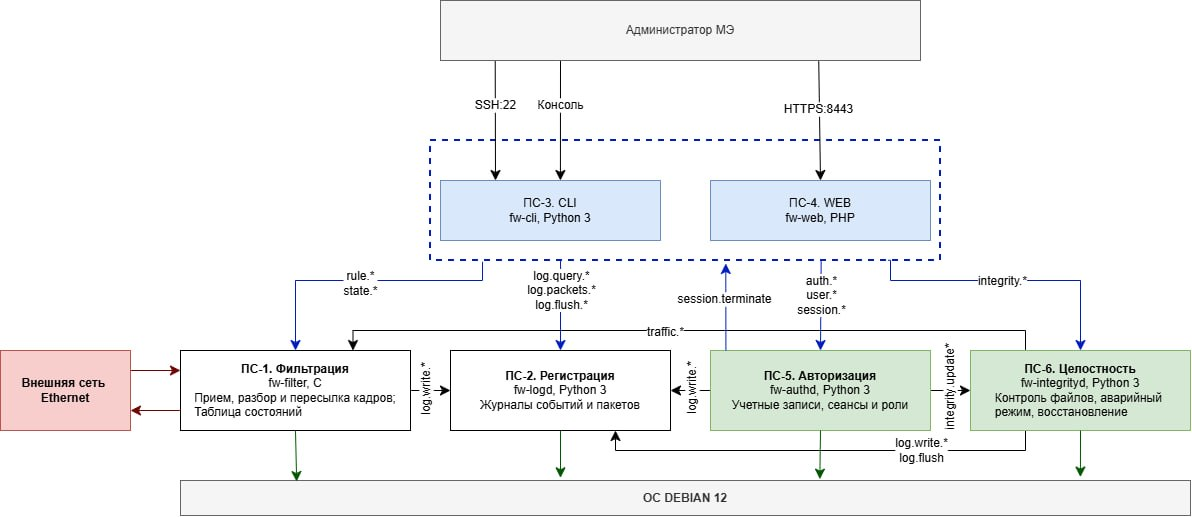
\includegraphics[width=0.95\textwidth]{arch.png}
		 \caption{Архитектура ПО МЭ: подсистемы и взаимодействие }
		 \end{figure}
	
	% \begin{figure}[H]
		% \centering
		% % \includegraphics[width=0.95\textwidth]{img/command_flow.png}
		% \caption{Обработка команды администратора}
		% \end{figure}
	%
	% \begin{figure}[H]
		% \centering
		% % \includegraphics[width=0.95\textwidth]{img/packet_flow.png}
		% \caption{Поток обработки пакета в ПС-1}
		% \end{figure}
	\subsection{Подсистемы}
	
	\begin{enumerate}
		\item 	\textbf{ПС-1 Фильтрация}
		
		\textbf{Назначение:} приём, разбор, фильтрация и пересылка кадров; таблица состояний.
		
		\textbf{Модули:} io (приём и отправка кадров), parser (разбор заголовков), rules (движок правил), conntrack (таблица состояний), pktlog\_client (передача записей в ПС-2).
		
		\textbf{Взаимодействие:} получает политику и команды контроля состояний от {ПС-3 и ПС-4}; команды блокировки от ПС-6; передаёт записи журнала пакетов в ПС-2.
		
		\textbf{Требования:} FR-01, FR-05 – FR-23.
		
		\textbf{Основной поток (обработка пакета):}
		\begin{enumerate}
			\item Принять кадр, разобрать заголовки Ethernet, IPv4 и TCP, UDP или ICMP.
			\item Если контроль состояний включён, найти запись таблицы состояний по ключу в прямом и обратном направлении.
			\item Запись найдена: проверить соответствие пакета состоянию и интерфейс поступления, обновить состояние и таймер, передать пакет — прямого направления на выходные интерфейсы записи, обратного на её входной интерфейс (FR-15).
			\item Запись не найдена: просматривать активные правила по возрастанию номера; «перейти к правилу N» продолжает просмотр с правила N.
			\item Если правило имеет атрибут «контролировать» и действие «передать», а пакет — допустимый первый пакет соединения (TCP SYN, первый UDP, ICMP Echo Request), создать запись с входным интерфейсом, выходными интерфейсами и номером правила.
			\item Если у правила установлен флаг регистрации, передать запись в ПС-2.
			\item Выполнить действие: передать или удалить.
		\end{enumerate}
		
		\textbf{Альтернативные потоки:}
		\begin{itemize}
			\item Ошибка разбора заголовка — кадр удаляется (FR-12). Кадр ARP или другого протокола Ethernet проверяется по правилам с полем \texttt{eth-proto}; если подходящего правила нет, ARP при включённой пересылке передаётся на все включённые интерфейсы, кроме входного, а прочие кадры удаляются (FR-11).
			\item Режим аварийной поддержки — кадр удаляется.
			\item Пакет не соответствует состоянию записи (вне контекста соединения) — пакет удаляется и регистрируется, если у правила записи установлен флаг регистрации (FR-22).
			\item Правило «контролировать» совпало, но пакет не может открывать соединение — пакет удаляется.
			\item Подходящего правила нет — пакет удаляется с номером правила 0 (FR-08).
		\end{itemize}
		
		\item \textbf{ПС-2 Регистрация}
		
		\textbf{Назначение:} ведение журналов событий и пакетов, выборки, ограничение размера.
		
		\textbf{Модули:} event\_log, packet\_log, query (выборки), rotation (ограничение размера, очистка).
		
		\textbf{Взаимодействие:} принимает записи от всех подсистем и запросы выборки от {ПС-3 и ПС-4}.
		
		\textbf{Требования:} FR-24 – FR-29, FR-39, FR-40.
		
		\textbf{Хранение журналов.} Журнал событий хранится в базе данных SQLite на диске и сохраняется при перезагрузке. Журнал пакетов хранится на диске в двоичном кольцевом файле из записей фиксированной длины; записи накапливаются в буфере в памяти и записываются в файл блоками~--- по заполнению блока или не реже раза в секунду. Такой подход снижает накладные расходы при интенсивном трафике. При аварийном отключении питания теряются только записи из буфера, ещё не записанные в файл (не более чем за 1~с).
		
		\item 	\textbf{ПС-3 CLI}
		
		\textbf{Назначение:} командный интерфейс (локальная консоль и SSH), выполнение команд, вывод результатов.
		
		\textbf{Модули:} repl (цикл чтения-выполнения), parser (разбор команд), formatter (вывод таблиц и страниц), session (локальный кэш роли).
		
		\textbf{Взаимодействие:} при входе — запрос к ПС-5; при выполнении команд — {вызовы ПС-1, ПС-2, ПС-6 напрямую (см. таблицу 12)}; уведомления об активности — в ПС-5.
		
		\textbf{Требования:} FR-02, FR-30 – FR-38, FR-44.
		
		\textbf{События:} E50 (отказ в доступе по роли) — в ПС-2.
		
		\item	\textbf{ПС-4 WEB}
		
		\textbf{Назначение:} web-интерфейс по HTTPS, форма входа, страницы разделов.
		
		\textbf{Модули:} server (PHP), auth (проверка сеанса), pages (разделы), api (вызовы {ПС-1, ПС-2, ПС-6}).
		
		\textbf{Взаимодействие:} при входе — запрос к ПС-5; при действиях — {вызовы ПС-1, ПС-2, ПС-6 напрямую (эквивалентно ПС-3, см. таблицу 12)}; уведомления об активности — в ПС-5.
		
		\textbf{Требования:} FR-03, FR-30 – FR-38, FR-44.
		
		\textbf{События:} E50 (отказ в доступе по роли) — в ПС-2.
		
		\textbf{ПС-5 Авторизация}
		
		\textbf{Назначение:} учётные записи, аутентификация, сеансы и роли.
		
		\textbf{Модули:} accounts, auth, sessions, roles.
		
		\textbf{Взаимодействие:} вызывается ПС-3 и ПС-4 при входе и для контроля активности; события передаёт в ПС-2.
		
		\textbf{Требования:} FR-30 – FR-37.
		
		\textbf{Основной поток (вход администратора):}
		\begin{enumerate}
			\item Принять идентификатор и пароль, проверить, не заблокирован ли вход.
			\item Сравнить хэш пароля с хранимым.
			\item Определить роль по учётной записи.
			\item Если роль «чтение/запись» и уже есть активный сеанс с этой ролью, понизить роль до «только чтение», вывести М04, зарегистрировать Е04.
			\item Создать сеанс, зарегистрировать Е01.
		\end{enumerate}
		
		\textbf{Альтернативные потоки:}
		\begin{itemize}
			\item Вход заблокирован — М12.
			\item Хэш не совпал — М02, Е03; после 5 неудач подряд — блокировка, М12, Е06 (FR-31).
		\end{itemize}
		
		\item \textbf{ПС-6 Целостность}
		
		\textbf{Назначение:} контроль целостности, режим аварийной поддержки, восстановление файлов.
		
		\textbf{Модули:} hasher (SHA-256), checker (периодическая проверка), emergency (режим аварийной поддержки), restore (восстановление).
		
		\textbf{Взаимодействие:} управляет блокировкой трафика в ПС-1 и режимом ПС-3 и ПС-4; события передаёт в ПС-2.
		
		\textbf{Требования:} FR-45 – FR-50.
		
		\textbf{Основной поток (проверка):}
		\begin{enumerate}
			\item По таймеру, при запуске или по запросу проверить HMAC файла эталонов и вычислить SHA-256 каждого контролируемого файла.
			\item Сравнить с эталоном. Все значения совпали — штатный режим.
		\end{enumerate}
		
		\textbf{Альтернативные потоки:}
		\begin{itemize}
			\item Значение или HMAC не совпали — передать ПС-1 команду блокировки трафика и очистки таблицы состояний, перевести ПС-3 и ПС-4 в режим аварийной поддержки {(обе подсистемы всегда, командой \texttt{emergency.enter})}, зарегистрировать Е40.
			\item После восстановления файла администратором проверка повторяется; при успехе блокировка снимается, режим становится штатным {(ПС-3 и ПС-4 получают \texttt{emergency.exit})}, регистрируется Е41.
		\end{itemize}
		
		\textbf{Формирование эталонов и резервных копий.} Эталонные контрольные суммы и резервные копии формируются до установки ПО~--- при сборке установочных пакетов в доверенной среде. Это исключает возможность подмены контролируемых файлов в момент расчёта эталонов. Резервные копии обновляются при каждом штатном изменении контролируемых файлов администратором.
		
	\end{enumerate}
	
	\subsection{Взаимодействие подсистем}
	{При входе администратора клиент (ПС-3 или ПС-4) взаимодействует с ПС-5 для аутентификации и определения роли (FR-37a); последующие команды выполняются с локально сохранённой ролью, а результат фиксируется в ПС-2.}
	
	Основные направления взаимодействия подсистем:
	\begin{itemize}
		\item ПС-3 и ПС-4 \textrightarrow{} ПС-5: {аутентификация при входе, управление учётными записями и сеансами, контроль активности (FR-37a)};
		\item ПС-3 и ПС-4 \textrightarrow{} ПС-1: управление политикой доступа и таблицей состояний;
		\item ПС-3 и ПС-4 \textrightarrow{} ПС-2: выборки журналов, очистка журнала пакетов;
		\item ПС-3 и ПС-4 \textrightarrow{} ПС-6: проверка целостности, восстановление файлов;
		\item ПС-1 \textrightarrow{} ПС-2: записи журнала пакетов, события E14 и E15;
		\item ПС-6 \textrightarrow{} ПС-1: блокировка трафика, очистка таблицы состояний; ПС-6 \textrightarrow{} ПС-3 и ПС-4: вход и выход из режима аварийной поддержки; {ПС-5 \textrightarrow{} ПС-3 и ПС-4: принудительное завершение сеанса (FR-35);}
		\item все подсистемы \textrightarrow{} ПС-2: события журнала (E01--E50).
	\end{itemize}
	
	Транспорт и формат сообщений приведены в п. 3.4, полный перечень команд подсистем --- в п. 3.5.
	\subsection{Системные функции (ОС)}
	
	Функции сетевых интерфейсов, маршрутов, даты и времени, питания и системной информации не выделяются в отдельную подсистему ПО МЭ, а выполняются операционной системой Debian 12. Доступ к ним осуществляется:
	\begin{itemize}
		\item из CLI — через утилиты ip, route, timedatectl, systemctl;
		\item из web-интерфейса — через те же утилиты, вызываемые из PHP;
		\item из других подсистем — через системные вызовы ОС.
	\end{itemize}
	
	ПС-3 и ПС-4 работают без привилегий администратора ОС. Для системных команд им разрешён запуск через sudo строго фиксированного списка команд (\texttt{ip}, \texttt{route}, \texttt{timedatectl}, \texttt{systemctl}): файл \texttt{/etc/sudoers.d/fw}, полные пути, допустимые аргументы, без запроса пароля, без интерпретации аргументов оболочкой. Команда запускается только после проверки роли «чтение/запись» (FR-32) и параметров (FR-42).
	
	Требования: FR-42, FR-43.
	
	\subsection{Проектные решения}
	
	\begin{itemize}
		\item \textbf{Прозрачный режим (L2).} ПС-1 принимает кадры на сокетах AF\_PACKET (TPACKET\_V3), применяет правила и отправляет разрешённые кадры на выходные интерфейсы из правила. Пересылка средствами ядра (ip\_forward) отключена. Так реализуются фильтрация по MAC-адресам и выбор выходных интерфейсов (ТЗ 2.2, 2.3). Интерфейсы работают в неразборчивом режиме; кадры, отправленные самим ПС-1, повторно не обрабатываются.
		
		\item \textbf{Управляющий трафик.} Кадры, адресованные самому МЭ (SSH, HTTPS), обрабатывает сетевой стек ОС. Доступ к управлению ограничивается списком управляющих интерфейсов и разрешённых адресов (таблица 3), а не правилами политики доступа. {ПС-1 не перехватывает кадры, у которых MAC-адрес получателя или IP-адрес назначения принадлежит самому МЭ: такие кадры остаются в сетевом стеке ОС и обрабатываются штатным механизмом приёма. ПС-1 обрабатывает только транзитные кадры.}
		
		
		\item \textbf{Хранение.} Форматы хранения приведены в таблице 6; пароли хэшируются алгоритмом PBKDF2-HMAC-SHA-256 с солью.
		
		\item \textbf{Применение политики.} При изменении политики ПС-1 не модифицирует действующую таблицу правил, а строит новую таблицу отдельно, проверяет её целостность и только после этого  подменяет указатель на активную таблицу (FR-10). Пакеты, обрабатываемые в момент подмены, используют либо старую, либо новую таблицу целиком — промежуточное состояние исключено. После подмены удаляются записи таблицы состояний, созданные изменёнными или удалёнными правилами (FR-23). Файл политики и его эталонный хэш при этом не изменяются: они обновляются только по команде config save, так же как для конфигурации (FR-41a, FR-47).
		
		\item \textbf{Запуск.} Подсистемы запускаются как службы systemd; перезагрузка подсистемы — перезапуск её службы. {Порядок запуска: \texttt{fw-integrityd} стартует до \texttt{fw-filter}; \texttt{fw-filter} стартует в режиме \texttt{emergency\_mode=1} (drop-all). Обработка трафика включается только после успешной проверки целостности: ПС-6 передаёт ПС-1 команду \texttt{traffic.unblock}, после чего ПС-3/ПС-4 загружают актуальную политику через \texttt{rule.replace}. Если integrity check не пройден, обработка трафика не включается (FR-04, FR-48).}
		
		\item \textbf{Сеанс администратора.} При входе администратора CLI взаимодействует с ПС-5 один раз: ПС-5 проверяет учётные данные, создаёт сеанс и возвращает CLI роль. В дальнейшем CLI хранит роль локально и выполняет команды без обращения к ПС-5. Для контроля таймаута CLI периодически уведомляет ПС-5 о факте выполнения команд. Это снижает накладные расходы на каждую команду и ускоряет работу администратора.
		
		\item \textbf{Сохранение политики.} Изменения политики доступа и параметров конфигурации, выполняемые командами, применяются к рабочей (текущей) конфигурации немедленно. Запись в файлы сохранённой конфигурации выполняется только по команде config save. При перезагрузке без сохранения загружается последняя сохранённая конфигурация. Политика доступа сохраняется тем же способом: команды rule add, rule edit, rule del, rule enable и rule disable сразу изменяют рабочую политику в ПС-1 (через \texttt{rule.replace}), а в файл политики она записывается только по команде config save, после чего обновляется эталонный хэш файла (\texttt{integrity.update\_baseline}). При перезагрузке без сохранения загружается последняя сохранённая политика.
	\end{itemize}
	
	\subsection{Командный интерфейс (CLI)}
	\textbf{Доступ.} CLI доступен локально (консоль МЭ) и удалённо (SSH, FR-02). После запуска выводится приглашение M01; пароль при вводе не отображается. После входа приглашение имеет вид admin@fw[rw]> или admin@fw[ro]>, в режиме аварийной поддержки — admin@fw[EMERGENCY]>.
	
	\textbf{Синтаксис.} Команда записывается как «группа действие [аргументы]». Позиционные аргументы указываются после действия, именованные — в виде имя=значение. Имена команд — строчными буквами. Значения с пробелами заключаются в двойные кавычки, списки разделяются запятой без пробелов, диапазоны — дефисом.
	
	\textbf{Форматы значений:} IPv4-адрес — 192.168.1.10, с маской 192.168.1.0/24, диапазон 192.168.1.10-192.168.1.20; MAC-адрес — AA:BB:CC:DD:EE:FF; порт — 80 или 1024-2000; дата и время — ГГГГ-ММ-ДД чч:мм:сс; интерфейс — имя из конфигурации (eth0…eth5).
	
	\textbf{Подтверждение.} Команды, отмеченные в таблице 7 знаком «*», запрашивают «Подтвердите (y/n):». Любой ответ, кроме y, отменяет операцию без изменений и без регистрации события.
	
	\textbf{Вывод.} Списки выводятся таблицей с заголовком, журналы — постранично, от новых записей к старым (страница задаётся аргументом page=N, по умолчанию 1). Пароли и хэши паролей не выводятся.
	
	\textbf{Служебные команды:} help — список групп команд; help группа — синтаксис команд группы; whoami — идентификатор, роль, интерфейс и IP-адрес текущего сеанса; logout или exit — завершение сеанса (E02).
	
	В таблице 7 столбец «Права» указывает минимальную роль (RO — обе роли, RW — только «чтение/запись»), столбец «Авар.» — доступна ли команда в режиме аварийной поддержки (недоступные отклоняются с M10), столбец «Web» — раздел web-интерфейса с той же функцией.

	\begin{xltabular}{\textwidth}{|p{3.2cm}|p{3cm}|c|p{2cm}|c|p{3cm}|}
		
		\caption{Команды CLI} \\
		\hline
		\textbf{Команда} & \textbf{Назначение} & \textbf{Права} & \textbf{Событие} & \textbf{Авар.} & \textbf{Web} \\
		\hline
		\endfirsthead
		
		\hline
		\multicolumn{6}{|l|}{\small\itshape Продолжение таблицы \thetable} \\
		\hline
		\textbf{Команда} & \textbf{Назначение} & \textbf{Права} & \textbf{Событие} & \textbf{Авар.} & \textbf{Web} \\
		\hline
		\endhead
		
		\hline
		\multicolumn{6}{r|}{\small\itshape Продолжение на следующей странице...} \\
		\endfoot
		
		\hline
		\endlastfoot
		
		\multicolumn{6}{|l|}{\textbf{Правила фильтрации (ТЗ 8.3)}} \\
		\hline
		rule list & Список правил со счётчиками срабатываний & RO & — & да & Политика доступа \\
		\hline
		rule show N & Все поля правила N & RO & — & да & Политика доступа \\
		\hline
		rule add N имя=значение ... & Добавить правило (аргументы — таблица 2) & RW & E20 / E50 / E43 & нет & Политика доступа \\
		\hline
		rule edit N имя=значение ... & Изменить поля правила & RW & E21 / E50 / E43 & нет & Политика доступа \\
		\hline
		rule enable N, rule disable N & Включить или отключить правило & RW & E21 / E50 / E43 & нет & Политика доступа \\
		\hline
		rule del N & Удалить правило (M11, если на него есть переход) & RW & E22 / E50 / E43 & нет & Политика доступа \\
		\hline
		
		\multicolumn{6}{|l|}{\textbf{Журналы (ТЗ 5.4–5.6)}} \\
		\hline
		log events show [code=] [from=] [to=] [page=N] & Просмотр и выборка журнала событий & RO & — & да & Журналы: события \\
		\hline
		log packets show [action={accept}\textbar{}drop] [in=] [out=] [rule=N] [smac=] [dmac=] [src=] [dst=] [sport=] [dport=] [from=] [to=] [page=N] & Просмотр и выборка журнала пакетов & RO & — & да & Журналы: пакеты \\
		\hline
		log packets clear * & Очистить журнал пакетов & RW & E34 / E50 / E43 & нет & Журналы: пакеты \\
		\hline
		
		\multicolumn{6}{|l|}{\textbf{Контроль состояний (ТЗ 9.7)}} \\
		\hline
		state status & Настройки механизма (включён ли, таймауты) & RO & — & да & Контроль состояний \\
		\hline
		state table & Таблица состояний & RO & — & да & Контроль состояний \\
		\hline
		state enable, state disable & Включить или отключить механизм & RW & E14, E15, E50 / E43 & нет & Контроль состояний \\
		\hline
		state delete ID & Удалить запись & RW & E35 / E50 / E43 & нет & Контроль состояний \\
		\hline
		state delete all * & Удалить все записи & RW & E35 / E50 / E43 & нет & Контроль состояний \\
		\hline
		
		\multicolumn{6}{|l|}{\textbf{Конфигурации (ТЗ 5.8)}} \\
		\hline
		config show current, config show saved & Вывести текущую или сохранённую конфигурацию & RO & — & да & Конфигурация \\
		\hline
		config save & Сохранить текущую конфигурацию {и политику доступа} & RW & E31 / E50 / E43 & нет & Конфигурация \\
		\hline
		config apply saved * & Применить сохранённую конфигурацию & RW & E31 / E50 / E43 & нет & Конфигурация \\
		\hline
		config apply default * & Применить конфигурацию по умолчанию & RW & E31 / E50 / E43 & нет & Конфигурация \\
		\hline
		config set имя=значение & Изменить параметр (таблица 3) & RW & E30 / E50 / E43 & нет & Конфигурация \\
		\hline
		
		\multicolumn{6}{|l|}{\textbf{Учётные записи и сеансы (ТЗ 5.9)}} \\
		\hline
		user list & База учётных записей без паролей & RO & — & да & Администраторы \\
		\hline
		user add ID role=rw\textbar{}ro & Добавить, пароль запрашивается скрытым вводом & RW & E32 / E50 / E43 & нет & Администраторы \\
		\hline
		user edit ID [role=rw\textbar{}ro] [password] & Изменить роль или пароль & RW & E32 / E50 / E43 & нет & Администраторы \\
		\hline
		user del ID * & Удалить учётную запись ({M05} для admin) & RW & E32, E07 / E50 / E43 & нет & Администраторы \\
		\hline
		session list & Активные сеансы & RO & — & да & Администраторы \\
		\hline
		session kill ID & Сбросить сеанс администратора & RW & E05 / E50 / E43 & нет & Администраторы \\
		\hline
		
		\multicolumn{6}{|l|}{\textbf{Интерфейсы Ethernet (ТЗ 5.10)}} \\
		\hline
		if list, if show ИМЯ & Состояние интерфейсов (адрес, список, счётчики) & RO & — & да & Сеть \\
		\hline
		if up ИМЯ, if down ИМЯ & Включить или выключить интерфейс & RW & E33 / E50 / E43 & нет & Сеть \\
		\hline
		if ip ИМЯ адрес/маска & Настроить IP-адрес интерфейса & RW & E33 / E50 / E43 & нет & Сеть \\
		\hline
		
		\multicolumn{6}{|l|}{\textbf{Система (ТЗ 5.11)}} \\
		\hline
		sys info & Процессор, память, интерфейсы, режим, состояние подсистем & RO & — & да & Состояние. Система \\
		\hline
		time show, time set "ДАТА ВРЕМЯ" & Просмотр и настройка даты и времени & RO / RW & E33 / E50 / E43 & да / нет & Система \\
		\hline
		route list & Системные маршруты & RO & — & да & Сеть \\
		\hline
		route add сеть/маска шлюз, route del сеть/маска & Добавить или удалить маршрут & RW & E33 / E50 / E43 & нет & Сеть \\
		\hline
		subsystem list & Состояние подсистем & RO & — & да & Система \\
		\hline
		subsystem restart ИМЯ * & Перезагрузить подсистему & RW & E13, E12 / E50 / E43 & нет & Система \\
		\hline
		sys reboot * & Перезагрузить устройство & RW & E11, E10 / E50 / E43 & нет & Система \\
		\hline
		sys shutdown * & Выключить устройство & RW & E11 / E50 / E43 & нет & Система \\
		\hline
		
		\multicolumn{6}{|l|}{\textbf{Контроль целостности (ТЗ 6)}} \\
		\hline
		integrity status & Результат последней проверки и режим & RO & — & да & Система \\
		\hline
		integrity check & Проверка целостности по запросу & RW & E42 / E50 / E43 & да & Система \\
		\hline
		integrity restore ФАЙЛ\textbar{}all & Восстановить файл из резервной копии & RW & E41 / E50 / E43 & да & Система \\
		\hline
		
		\multicolumn{6}{|l|}{\textbf{Служебные}} \\
		\hline
		help, whoami, logout, exit & См. выше & RO & E02 (logout) & да & Шапка страницы \\
		\hline
		
	\end{xltabular}
	
	\subsection{Web-интерфейс}
	Web-интерфейс доступен только по HTTPS (самоподписанный сертификат создаётся при установке) на адресах управляющих интерфейсов и локально по адресу 127.0.0.1. Язык интерфейса — русский. {Web-интерфейс вызывает те же команды (см. таблицу 7, столбец «Web»), что и CLI (FR-38); отличие — источник сообщений (\texttt{"src":"web"}) и транспорт входа (HTTPS).}
	
	Все страницы, кроме формы входа, содержат:
	\begin{itemize}
		\item шапку: идентификатор, роль, IP-адрес, индикатор режима («Штатный» / «Аварийная поддержка»), кнопку «Выход»;
		\item левое меню разделов;
		\item область сообщений: ошибки выводятся красным, M09 — зелёным; при M04 и M08 вверху страницы показывается постоянный баннер;
		\item рабочую область: таблица данных, фильтры, формы и кнопки действий раздела.
	\end{itemize}
	
	Разделы меню:
	\begin{itemize}
		\item Вход — поля «Идентификатор» и «Пароль», кнопка «Войти»; после входа открывается раздел «Состояние».
		\item \textbf{Состояние} — режим работы, состояние подсистем, включён ли контроль состояний, число правил и записей таблицы состояний, состояние интерфейсов, результат последней проверки целостности, права текущего сеанса.
		\item \textbf{Политика доступа} — таблица правил, отсортированная по номеру, с переключателем активности в строке; форма правила (таблица 2).
		\item \textbf{Контроль состояний} — переключатель механизма, таймауты, таблица состояний.
		\item \textbf{Журналы — «События» и «Пакеты»:} фильтры по критериям FR-39, постраничная таблица; кнопка очистки журнала пакетов.
		\item \textbf{Конфигурация} — вкладки «Текущая» и «Сохранённая», действия с конфигурациями, форма параметров (таблица 3).
		\item \textbf{Администраторы} — учётные записи (форма: идентификатор, пароль с повтором, роль) и активные сеансы.
		\item \textbf{Сеть} — интерфейсы и маршруты.
		\item \textbf{Система} — информация, дата и время, целостность (список контролируемых файлов со статусом, в аварийном режиме — кнопки восстановления), подсистемы, перезагрузка и выключение.
	\end{itemize}
	
	Для роли «только чтение» кнопки изменения не отображаются; изменяющий запрос, отправленный напрямую, отклоняется с M03.
	
	В режиме аварийной поддержки доступны только разделы «Состояние», «Журналы», «Конфигурация» (просмотр) и «Система»; остальные запросы отклоняются с M10.
	
	Действия, требующие подтверждения в CLI, в web-интерфейсе тоже требуют подтверждения.
	
	
	\section{Разработка ПО МЭ}
	В разделе описывается программная реализация ПО МЭ: технологии и среда разработки, структура проекта и размещение файлов, правила разработки, интерфейсы взаимодействия подсистем и структуры данных.
	\subsection{Технологии и среда}

	\begin{xltabular}{\textwidth}{|X|X|}
		\caption{Технологии и среда} \\
		\hline
		\textbf{Параметр} & \textbf{Значение} \\
		\hline
		\endfirsthead
		\hline
		\multicolumn{2}{|l|}{\small\itshape Продолжение таблицы \thetable} \\
		\hline
		\textbf{Параметр} & \textbf{Значение} \\
		\hline
		\endhead
		\hline
		\multicolumn{2}{r|}{\small\itshape Продолжение на следующей странице...} \\
		\endfoot
		\hline
		\endlastfoot
		Язык ПС-1 & C \\
		\hline
		Язык ПС-2 {, ПС-3, ПС-5, ПС-6} & Python 3  \\
		\hline
		Язык ПС-4 (WEB) & PHP , HTTPS через nginx \\
		\hline
		Сборка & make, gcc; для Python — venv и файл зависимостей \\
		\hline
		Среда исполнения & Debian 12, x86\_64, systemd \\
		\hline
		Библиотеки & SQLite (модуль sqlite3 Python), OpenSSL (HTTPS) \\
		\hline
		Система контроля версий & Git \\
		\hline
		Привилегии & Каждая подсистема работает от отдельного непривилегированного пользователя ОС: fw-filter (ПС-1, дополнительно право CAP\_NET\_RAW), fw-logd (ПС-2), fw-cli (ПС-3), fw-web (ПС-4), {fw-authd} (ПС-5), {fw-integrityd} (ПС-6). Ни одна подсистема не работает от root; файлы каждой подсистемы принадлежат её пользователю (таблица «Размещение файлов ПО МЭ»). Действия, требующие прав root, выполняются через sudo по фиксированному списку команд: системные команды ПС-3 и ПС-4 (см. «Системные функции (ОС)») и замена контролируемых файлов при восстановлении (ПС-6) \\
		\hline
	\end{xltabular}
	
	
	\subsection{Структура проекта и размещение файлов}
	Проект разбит на каталоги подсистем (fw-filter, fw-logd, fw-cli, fw-web, fw-authd, fw-integrityd).
	
	Кроме каталогов подсистем, проект содержит: common/ (протокол сообщений, формат правил, коды событий и сообщений), etc/ (конфигурация по умолчанию, политика, службы systemd), tests/ (модульные и функциональные тесты, скрипты стенда), docs/ (спецификация, ПМИ, руководство администратора).
	
	\textbf{Размещение файлов ПО МЭ}
	
	Ниже перечислены файлы и каталоги ПО МЭ, их владельцы и права доступа. ПС-6 получает право чтения всех контролируемых файлов через ACL (\texttt{setfacl}), чтобы вычислять их хэши; записывать в них она может только при восстановлении через sudo. Всего контролируется около 40 файлов; предельное число задаётся константой \texttt{MAX\_CONTROLLED\_FILES} = 64, список путей хранится в конфигурации ПС-6.
	
	\begin{xltabular}{\linewidth}{|p{4.3cm}|X|p{3cm}|p{2.1cm}|}
		\caption{Размещение файлов ПО МЭ} \\
		\hline
		\textbf{Путь} & \textbf{Содержимое} & \textbf{Владелец, права} & \textbf{Контроль} \\
		\hline
		\endfirsthead
		\hline
		\multicolumn{4}{|l|}{\small\itshape Продолжение таблицы \thetable} \\
		\hline
		\textbf{Путь} & \textbf{Содержимое} & \textbf{Владелец, права} & \textbf{Контроль} \\
		\hline
		\endhead
		\hline
		\multicolumn{4}{r|}{\small\itshape Продолжение на следующей странице...} \\
		\endfoot
		\hline
		\endlastfoot
		\texttt{/usr/lib/fw/bin/}\newline\texttt{fw-filter} & Исполняемый файл ПС-1 & root, 0755 & да \\
		\hline
		\texttt{/usr/lib/fw/}\newline\texttt{\{logd,cli,authd,}\newline\texttt{integrityd\}/} & Модули ПС-2, ПС-3, ПС-5, ПС-6 (Python) & root, 0644 & да \\
		\hline
		\texttt{/usr/share/fw/web/} & Файлы ПС-4 (PHP) & root, 0644 & да \\
		\hline
		\texttt{/etc/systemd/system/}\newline\texttt{fw-*.service} & Скрипты запуска подсистем & root, 0644 & да \\
		\hline
		\texttt{/etc/sudoers.d/fw} & Фиксированный список команд sudo & root, 0440 & да \\
		\hline
		\texttt{/etc/fw/*.json} & Сохранённая конфигурация подсистем & fw-cli, группа fw-mgmt (fw-cli, fw-web), 0660 & да \\
		\hline
		\texttt{/etc/fw/policy.json} & Сохранённая политика доступа & {fw-cli, группа fw-mgmt (fw-cli, fw-web, fw-filter), 0640} & да \\
		\hline
		\texttt{/etc/fw/default/} & Конфигурация и политика по умолчанию & root, 0644 & да \\
		\hline
		\texttt{/etc/fw/}\newline\texttt{accounts.json} & Учётные записи администраторов & {fw-authd}, 0600 & да \\
		\hline
		\texttt{/etc/fw/hmac.key} & Ключ HMAC файла эталонов & {fw-integrityd}, 0400 & нет \\
		\hline
		\texttt{/var/lib/fw/}\newline\texttt{baseline.json} & Эталонные хэши SHA-256 контролируемых файлов & {fw-integrityd}, 0600 & защищён HMAC \\
		\hline
		\texttt{/var/lib/fw/backup/} & Резервные копии контролируемых файлов & {fw-integrityd}, 0700 & сверяются с эталоном \\
		\hline
		\texttt{/var/lib/fw/}\newline\texttt{events.db} & Журнал событий (SQLite) & fw-logd, 0600 & нет \\
		\hline
		\texttt{/var/lib/fw/}\newline\texttt{packets.bin} & Журнал пакетов (двоичный файл) & fw-logd, 0600 & нет \\
		\hline
	\end{xltabular}
	\subsection{Правила разработки}

	\begin{itemize}
		\item Коды событий и сообщений определяются один раз в common/ и совпадают с таблицами 4 и 5.
		\item Все данные от администратора и из сети проверяются на входе подсистемы; данным другой подсистемы без проверки не доверяют.
		\item Ошибки возвращаются кодом и сообщением из таблицы 5; необработанные исключения не завершают процесс подсистемы.
		\item Каждый модуль имеет модульные тесты.
		\item Правила проверки данных (таблицы 2 и 3, FR-13, FR-36, FR-39) описываются один раз в \texttt{common/validation.json} и реализуются в ПС-3 (Python) и ПС-4 (PHP) строго по этому описанию. Для обоих интерфейсов используется общий набор тестовых сценариев (\texttt{tests/shared/}); результаты проверок и сообщения об ошибках должны совпадать.
		\item Каждый исходный файл начинается с шапки по единому шаблону. Шаблон шапки:
	\end{itemize}
	
	\begin{alltt}
		/**
		* Система:     ПО межсетевого экрана (ПО МЭ)
		* Подсистема: <имя подсистемы, например ПС-1 Фильтрация>
		* Модуль:      <имя модуля, например parser>
		* Назначение:  <краткое описание назначения модуля>
		* Методы:
		*   - <имя метода 1> — <назначение>
		*   - <имя метода 2> — <назначение>
		*/
	\end{alltt}
	
	Разработчик подсистемы самостоятельно пишет программу и методику испытаний для своей подсистемы и проводит испытания.
	
	\subsection{Интерфейсы взаимодействия подсистем}
	
	\textbf{Транспорт и формат сообщений}
	
	Все подсистемы общаются через локальные Unix-сокеты (AF\_UNIX, SOCK\_STREAM) в формате JSON-сообщений, разделяемых символом перевода строки (\texttt{\textbackslash n}). Для событий, генерируемых с высокой частотой (журнал пакетов), используется бинарный формат фиксированной длины.
	
{Каждый сокет имеет путь \texttt{/run/fw/<subsystem>.sock}, владельца~--- соответствующий пользователь ОС, и права доступа \texttt{0660} с группой \texttt{fw-mgmt}, в которую входят все пользователи подсистем~\texttt{fw-*}. Доступ со стороны посторонних процессов исключается.}
	
	\textbf{Формат JSON-сообщения}
	
	Любое сообщение имеет единый формат:
	
	\begin{lstlisting}[language=Java, caption={Конверт сообщения}, label={lst:envelope}]
		{
			"msg_id": 1042,               // уникальный идентификатор сообщения
			"type": "request",            // request | response | event
			"src": "cli",                 // источник: cli | web | filter | logd | authd | integrityd | os
			"dst": "authd",               // получатель
			"cmd": "auth.login",          // имя команды (п. 3.5)
			"ts": "2026-03-14T10:21:33.482Z",
			"payload": { ... },           // тело команды (зависит от cmd)
			"reply_to": null              // для type=response: msg_id запроса
		}
	\end{lstlisting}
	
	\textbf{Ответ} на команду:
	
	\begin{lstlisting}[language=Java, caption={Ответ}, label={lst:response}]
		{
			"msg_id": 1043,
			"type": "response",
			"src": "authd", "dst": "cli",
			"reply_to": 1042,
			"status": "ok",               // ok | error
			"error_code": null,           // M01..M16 при status=error
			"error_message": null,
			"payload": { "session_id": "...", "role": "rw" }
		}
	\end{lstlisting}
	
	\textbf{Событие} (односторонняя отправка в ПС-2 и от ПС-6):
	
	\begin{lstlisting}[language=Java, caption={Событие}, label={lst:event}]
		{
			"msg_id": 1044, "type": "event",
			"src": "filter", "dst": "logd",
			"cmd": "log.write.event",
			"payload": { "event_code": "E20", "result": "ok", ... }
		}
	\end{lstlisting}
	
	\textbf{Общие правила}
	\begin{itemize}
		\item Все строки~--- UTF-8, ограничены 255 символами, если в структуре не указано иное.
		\item IPv4-адреса~--- строка в формате \texttt{"a.b.c.d"} или \texttt{"a.b.c.d/len"}.
		\item MAC-адреса~--- строка \texttt{"AA:BB:CC:DD:EE:FF"}.
		\item Время~--- ISO~8601 с миллисекундами.
		\item Таймаут ожидания ответа~--- 5~с. Если ответ не получен, клиент повторяет запрос ещё до двух раз с тем же \texttt{msg\_id}; получатель по \texttt{msg\_id} распознаёт повтор и возвращает прежний ответ, не выполняя команду повторно. Если ответа нет и после повторов, команда считается неуспешной: администратору выводится M16, в журнал событий записывается неуспешный результат с причиной (FR-28). События (\texttt{type=event}) подтверждения не требуют; если ПС-2 недоступна, отправитель хранит события в очереди в памяти (до 1000) и повторяет отправку каждые 5~с. {Для высокочастотного потока \texttt{log.write.packet} очередь не используется: ПС-1 буферизует не более 4096 записей; при переполнении новые записи отбрасываются, счётчик отброшенных записей доступен в ПС-1 по команде \texttt{stats.get}.}
	\end{itemize}
	
	\subsection{Команды подсистем}
	
	Ниже приведён полный перечень команд, которые каждая подсистема принимает и отправляет. Формат «\texttt{cmd (payload) → результат}».

	\begin{enumerate}
		\item	\textbf{ПС-1 Фильтрация }
		
		\textbf{Принимает:}
		\begin{xltabular}{\textwidth}{|p{4.2cm}|X|p{3.5cm}|}
			\caption{Входящие команды ПС-1} \\
			\hline
			\textbf{Команда} & \textbf{Назначение} & \textbf{Источник} \\
			\hline
			\endfirsthead
			\hline
			\multicolumn{3}{|l|}{\small\itshape Продолжение таблицы \thetable} \\
			\hline
			\textbf{Команда} & \textbf{Назначение} & \textbf{Источник} \\
			\hline
			\endhead
			\hline
			\multicolumn{3}{r|}{\small\itshape Продолжение на следующей странице...} \\
			\endfoot
			\hline
			\endlastfoot
			\texttt{rule.replace} & Атомарно заменить всю таблицу правил (счётчики срабатываний неизменённых правил сохраняются), {считав упакованные правила из файла по указанному пути} & ПС-3, ПС-4 \\
			\hline
			\texttt{rule.get} & Вернуть текущую таблицу правил со счётчиками срабатываний & ПС-3, ПС-4 \\
			\hline
			\texttt{state.enable} & Включить механизм контроля состояний & ПС-3, ПС-4 \\
			\hline
			\texttt{state.disable} & Отключить механизм, очистить таблицу & ПС-3, ПС-4 \\
			\hline
			\texttt{state.list} & Вернуть таблицу состояний & ПС-3, ПС-4 \\
			\hline
			\texttt{state.delete} & Удалить запись по ID & ПС-3 \\
			\hline
			\texttt{state.delete\_all} & Удалить все записи & ПС-3, ПС-4 \\
			\hline
			\texttt{state.status} & Вернуть настройки механизма & ПС-3, ПС-4 \\
			\hline
			\texttt{traffic.block} & Заблокировать весь транзитный трафик & ПС-6 \\
			\hline
			\texttt{traffic.unblock} & Снять блокировку & ПС-6 \\
			\hline
			\texttt{state.clear} & Принудительно очистить таблицу состояний & ПС-6 \\
			\hline
			\texttt{stats.get} & Вернуть счётчики пакетов и ошибок & ПС-3 \\
			\hline
		\end{xltabular}
		
		\textbf{Отправляет (события и пакеты):}
		\begin{itemize}
			\item \texttt{log.write.packet} - ПС-2 (бинарный формат: время, действие над пакетом, номер сработавшего правила, идентификатор соединения, входной и выходные интерфейсы, адреса и порты~--- см. «Запись журнала пакетов»).
			\item \texttt{log.write.event} - ПС-2 (E14, E15 ).
		\end{itemize}
		
		\item	\textbf{ПС-2 Регистрация }

		 
		 \textbf{Принимает:}
		\begin{xltabular}{\textwidth}{|p{4.2cm}|X|p{3.5cm}|}
			\caption{Входящие команды ПС-2} \\
			\hline
			\textbf{Команда} & \textbf{Назначение} & \textbf{Источник} \\
			\hline
			\endfirsthead
			\hline
			\multicolumn{3}{|l|}{\small\itshape Продолжение таблицы \thetable} \\
			\hline
			\textbf{Команда} & \textbf{Назначение} & \textbf{Источник} \\
			\hline
			\endhead
			\hline
			\multicolumn{3}{r|}{\small\itshape Продолжение на следующей странице...} \\
			\endfoot
			\hline
			\endlastfoot
			\texttt{log.write.event} & Записать событие в журнал & Все ПС \\
			\hline
			\texttt{log.write.packet} & Записать пакет (бинарный) & ПС-1 \\
			\hline
			\texttt{log.query.events} & Выборка событий по фильтру & ПС-3, ПС-4 \\
			\hline
			\texttt{log.query.packets} & Выборка пакетов по фильтру & ПС-3, ПС-4 \\
			\hline
			\texttt{log.packets.clear} & Очистить журнал пакетов & ПС-3, ПС-4 \\
			\hline
			\texttt{log.flush} & Сбросить буфер пакетов на диск & ПС-3 (при shutdown), ПС-6 \\
			\hline
		\end{xltabular}
		
		\textbf{Отправляет:}
		\begin{itemize}
			\item \texttt{log.write.event} - self (E36 при переполнении журнала пакетов, E37 при переполнении журнала событий).
		\end{itemize}
		
		\item	\textbf{ПС-3 CLI }
		
		ПС-3 работает как клиент и не имеет входящих команд управления. Она отправляет запросы в ПС-1, ПС-2, ПС-5, ПС-6 и ОС. {Единственные входящие сообщения ПС-3~--- служебные уведомления ПС-6 о смене режима работы и ПС-5 о завершении сеанса (таблица ниже); они не являются командами управления и не зависят от того, в каком интерфейсе открыт сеанс администратора.}


		{\textbf{Принимает:}}
		\begin{xltabular}{\textwidth}{|p{3.8cm}|X|p{3.2cm}|}
			\caption{Входящие команды ПС-3} \\
			\hline
			\textbf{Команда} & \textbf{Назначение} & \textbf{Источник} \\
			\hline
			\endfirsthead
			\hline
			\multicolumn{3}{|l|}{\small\itshape Продолжение таблицы \thetable} \\
			\hline
			\textbf{Команда} & \textbf{Назначение} & \textbf{Источник} \\
			\hline
			\endhead
			\hline
			\multicolumn{3}{r|}{\small\itshape Продолжение на следующей странице...} \\
			\endfoot
			\hline
			\endlastfoot
			\texttt{emergency.enter} & {Перейти в режим аварийной поддержки: приглашение \texttt{admin@fw[EMERGENCY]>}, команды, недоступные в этом режиме (таблица 7, столбец «Авар.»), отклоняются с M10 (FR-49)} & ПС-6 \\
			\hline
			\texttt{emergency.exit} & {Вернуться в штатный режим: приглашение \texttt{admin@fw[rw]>} или \texttt{admin@fw[ro]>} по роли сеанса} & ПС-6 \\
			\hline
			\texttt{session.terminate} & {Принудительно завершить сеанс: вывести М15 и завершить работу (FR-35)} & ПС-5 \\
			\hline
		\end{xltabular}

		{Каждый процесс ПС-3 (консоль или сеанс SSH) запускается отдельно и может не получить уведомление, отправленное до его запуска. Поэтому при старте, после входа администратора и перед выполнением каждой команды ПС-3 запрашивает у ПС-6 текущий режим командой \texttt{integrity.status}. Если ПС-6 не отвечает (M16), ПС-3 считает режим аварийным. Повторные \texttt{emergency.enter} в аварийном режиме и \texttt{emergency.exit} в штатном не меняют состояния и подтверждаются успешным ответом.}


		\textbf{Отправляет:}
		\begin{xltabular}{\textwidth}{|p{3.8cm}|X|p{3.2cm}|}
			\caption{Команды, отправляемые ПС-3} \\
			\hline
			\textbf{Команда} & \textbf{Назначение} & \textbf{Получатель} \\
			\hline
			\endfirsthead
			\hline
			\multicolumn{3}{|l|}{\small\itshape Продолжение таблицы \thetable} \\
			\hline
			\textbf{Команда} & \textbf{Назначение} & \textbf{Получатель} \\
			\hline
			\endhead
			\hline
			\multicolumn{3}{r|}{\small\itshape Продолжение на следующей странице...} \\
			\endfoot
			\hline
			\endlastfoot
			\texttt{auth.login} & Аутентификация, создание сеанса & ПС-5 \\
			\hline
			\texttt{auth.logout} & Завершение сеанса & ПС-5 \\
			\hline
			\texttt{auth.ping} & Уведомление об активности (таймаут) & ПС-5 \\
			\hline
			\texttt{user.*}, \texttt{session.*} & Управление учётными записями & ПС-5 \\
			\hline
			\texttt{rule.*} & Управление политикой & ПС-1 \\
			\hline
			\texttt{state.*} & Управление таблицей состояний & ПС-1 \\
			\hline
			\texttt{log.query.*}, \texttt{log.packets.clear} & Работа с журналами & ПС-2 \\
			\hline
			\texttt{integrity.*} & Работа с целостностью & ПС-6 \\
			\hline
			\texttt{config.*} & Работа с конфигурацией & self (в файлы), ПС-1, ПС-5, ПС-6 \\
			\hline
			\texttt{if.*}, \texttt{route.*}, \texttt{time.*}, \texttt{sys.*} & Системные команды & ОС (через системные вызовы и утилиты) \\
			\hline
		\end{xltabular}
		
		\item	\textbf{ПС-4 WEB }
		
		С точки зрения интерфейсов ПС-4 полностью эквивалентна ПС-3: те же команды, те же получатели {и те же входящие сообщения: ПС-4 принимает от ПС-6 \texttt{emergency.enter} и \texttt{emergency.exit}, от ПС-5~--- \texttt{session.terminate} (см. таблицу «Входящие команды ПС-3»). Режим работы ПС-4 дополнительно проверяет запросом \texttt{integrity.status} при каждом web-запросе, так как запросы обрабатываются независимыми процессами PHP; недоступные в аварийном режиме запросы отклоняются с M10}. Отличие~--- источник сообщений (\texttt{"src":"web"} вместо \texttt{"src":"cli"}) и транспорт входа (HTTPS от браузера).
		
		\item	\textbf{ПС-5 Авторизация }

		 
		 \textbf{Принимает:}
		\begin{xltabular}{\textwidth}{|p{3.8cm}|X|p{3.2cm}|}
			\caption{Входящие команды ПС-5} \\
			\hline
			\textbf{Команда} & \textbf{Назначение} & \textbf{Источник} \\
			\hline
			\endfirsthead
			\hline
			\multicolumn{3}{|l|}{\small\itshape Продолжение таблицы \thetable} \\
			\hline
			\textbf{Команда} & \textbf{Назначение} & \textbf{Источник} \\
			\hline
			\endhead
			\hline
			\multicolumn{3}{r|}{\small\itshape Продолжение на следующей странице...} \\
			\endfoot
			\hline
			\endlastfoot
			\texttt{auth.login} & Проверить пару id/пароль, создать сеанс & ПС-3, ПС-4 \\
			\hline
			\texttt{auth.logout} & Завершить сеанс & ПС-3, ПС-4 \\
			\hline
			\texttt{auth.ping} & Обновить время последней активности & ПС-3, ПС-4 \\
			\hline
			\texttt{user.list} & Список учётных записей & ПС-3, ПС-4 \\
			\hline
			\texttt{user.add} & Добавить учётную запись & ПС-3, ПС-4 \\
			\hline
			\texttt{user.edit} & Изменить роль или пароль & ПС-3, ПС-4 \\
			\hline
			\texttt{user.delete} & Удалить учётную запись & ПС-3, ПС-4 \\
			\hline
			\texttt{session.list} & Список активных сеансов & ПС-3, ПС-4 \\
			\hline
			\texttt{session.kill} & Принудительно завершить сеанс & ПС-3, ПС-4 \\
			\hline
		\end{xltabular}
		
		\textbf{Отправляет (события):} E01–E07, E32, E50 - ПС-2. {Также отправляет \texttt{session.} \texttt{terminate} в ПС-3/ПС-4 при принудительном завершении сеанса (FR-35) и \texttt{integ} \texttt{rity.update\_baseline} в ПС-6 после операций \texttt{user add}, \texttt{user edit}, \texttt{user delete}.}
		
		\item	\textbf{ПС-6 Целостность (fw-integrityd)}

		 
		 \textbf{Принимает:}
		\begin{xltabular}{\textwidth}{|p{3.8cm}|X|p{3.2cm}|}
			\caption{Входящие команды ПС-6} \\
			\hline
			\textbf{Команда} & \textbf{Назначение} & \textbf{Источник} \\
			\hline
			\endfirsthead
			\hline
			\multicolumn{3}{|l|}{\small\itshape Продолжение таблицы \thetable} \\
			\hline
			\textbf{Команда} & \textbf{Назначение} & \textbf{Источник} \\
			\hline
			\endhead
			\hline
			\multicolumn{3}{r|}{\small\itshape Продолжение на следующей странице...} \\
			\endfoot
			\hline
			\endlastfoot
			\texttt{integrity.check} & Принудительная проверка & ПС-3, ПС-4 \\
			\hline
			\texttt{integrity.status} & Результат последней проверки & ПС-3, ПС-4 \\
			\hline
			\texttt{integrity.restore} & Восстановить файл из резервной копии & ПС-3, ПС-4 \\
			\hline
			\texttt{integrity.}\newline\texttt{update\_baseline} & Обновить эталон {и резервную копию после штатного изменения}  & ПС-3, ПС-4 (автоматически при \texttt{config save}); ПС-5 (при \texttt{user add}, \texttt{user edit}, \texttt{user delete}) \\
			\hline
		\end{xltabular}
		
		\textbf{Отправляет:}
		\begin{itemize}
			\item \texttt{traffic.block}, \texttt{traffic.unblock}, \texttt{state.clear} - ПС-1.
			\item \texttt{emergency.enter}, \texttt{emergency.exit} - {ПС-3 и ПС-4 одновременно, независимо от того, в каком интерфейсе открыт сеанс администратора} (для смены приглашения и запрета команд). {Сообщения отправляются как запросы с ответом; недоступность одного получателя не задерживает отправку другому. При отсутствии ответа ПС-6 повторяет запрос с тем же \texttt{msg\_id} (до двух раз), регистрирует неуспешный результат (FR-28) и повторяет отправку, пока режим не подтверждён обоими получателями.}
			\item \texttt{log.write.event} (E40, E41, E42) - ПС-2.
		\end{itemize}
		
	\end{enumerate}
	\subsection{Структуры конфигурации подсистем}
	
	Каждая подсистема имеет собственную структуру конфигурации, которая считывается при старте из файлов JSON в \texttt{/etc/fw/}. Ниже приведены C-совместимые заголовки (в Python они реализуются как \texttt{dataclass}, в PHP~--- как ассоциативные массивы).
	
	\begin{enumerate}
		
		\item{Общие типы (common/types.h)}
		
		\begin{lstlisting}[language=C, caption={Общие типы}]
			#define MIN_INTERFACES     1
			#define MAX_INTERFACES     6
			#define MAX_CONTROLLED_FILES 64
			{\#define MAX\_PORT\_RANGES 8}
			#define MAX_IFACE_NAME     16
			#define MAX_RULES          65535
			#define MAX_COMMENT_LEN    256
			#define MAX_CMD_LEN        128
			#define MAX_PATH_LEN       256
			
			typedef uint16_t rule_id_t;
			typedef uint32_t ip4_t;
			typedef uint64_t mac_t;
			typedef uint64_t timestamp_us_t;
			
			{typedef struct \{ uint16\_t lo; uint16\_t hi; \} port\_range\_t;}
			{typedef struct \{ uint8\_t count; port\_range\_t r[MAX\_PORT\_RANGES]; \} port\_set\_t;}
			
			typedef enum { ACTION_ACCEPT, ACTION_GOTO, ACTION_DROP } action_t;
			typedef enum { ETH_PROTO_ANY, ETH_PROTO_ARP, ETH_PROTO_OTHER } eth_proto_t;
			typedef enum { ROLE_RO, ROLE_RW } role_t;
			typedef enum { RESULT_OK, RESULT_FAIL } result_t;
		\end{lstlisting}
		
		\item{Конфигурация ПС-1 (filter\_config.h)}
		
		Минимальное число интерфейсов~--- 1 (\texttt{MIN\_INTERFACES}, ТЗ 1.2). При одном интерфейсе МЭ доступен для управления, но транзитный трафик не пересылает, так как входной интерфейс не может быть выходным; для фильтрации транзитного трафика требуется не менее двух интерфейсов.
		
		\begin{lstlisting}[language=C, caption={filter\_config.h}]
			typedef struct {
				char   name[MAX_IFACE_NAME];  // eth0..eth5
				ip4_t  addr;                  // может быть 0 для транзитного
				ip4_t  mask;
				uint8_t enabled;
				uint8_t is_mgmt;              // 1 = управляющий интерфейс
			} iface_config_t;
			
			typedef struct {
				uint32_t tcp_syn_timeout_sec;   // 5
				uint32_t tcp_est_timeout_sec;   // 3600
				uint32_t tcp_fin_timeout_sec;   // 30
				{uint32\_t udp\_timeout\_no\_reply;  // 15}
				{uint32\_t udp\_timeout\_reply;     // 60}
				uint32_t icmp_timeout_sec;      // 5
				uint32_t state_table_size;      // 65536
				uint8_t  conntrack_enabled;     // 1
				uint8_t  arp_forwarding;        // 0
			} conntrack_config_t;
			
			typedef struct {
				iface_config_t     ifaces[MAX_INTERFACES];
				uint8_t            iface_count;       // MIN_INTERFACES..MAX_INTERFACES (1..6)
				conntrack_config_t conntrack;
				rule_t             rules[MAX_RULES];
				uint32_t           rule_count;
				uint8_t            emergency_mode;    // 0/1
			} filter_config_t;
		\end{lstlisting}
		
		\item{Конфигурация ПС-2 (logd\_config.h)}
		
		\begin{lstlisting}[language=C, caption={logd\_config.h}]
			typedef struct {
				char   events_db_path[MAX_PATH_LEN];   // /var/lib/fw/events.db
				uint64_t events_max_bytes;             // 50 * 1024 * 1024
				char   packets_dump_path[MAX_PATH_LEN];// /var/lib/fw/packets.bin
				uint64_t packets_max_bytes; // 100 * 1024 * 1024 = 104857600: ~1,9 млн записей по 55 байт; файл кольцевой
				uint32_t packets_block_records; // 4096: число записей в блоке записи на диск
				uint32_t packets_flush_interval_ms; // 1000: неполный блок записывается не реже раза в секунду
			} logd_config_t;
		\end{lstlisting}
		
		\item{Конфигурация ПС-3 (cli\_config.h)}
		
		\begin{lstlisting}[language=C, caption={cli\_config.h}]
			typedef struct {
				uint16_t page_size;              // 20
				uint8_t  color_enabled;          // 1
				uint32_t session_timeout_sec;    // 900 (15 минут)
			{uint32\_t ping\_interval\_sec;      // 60: минимальный интервал между auth.ping; уведомления отправляются только после выполнения команд, а не по таймеру — таймаут бездействия работает корректно}
				char     history_path[MAX_PATH_LEN];
			} cli_config_t;
		\end{lstlisting}
		
		\item{Конфигурация ПС-4 (web\_config.h)}
		
		\begin{lstlisting}[language=C, caption={web\_config.h}]
			typedef struct {
				uint16_t https_port;             // 8443
				char     cert_path[MAX_PATH_LEN];
				char     key_path[MAX_PATH_LEN];
				uint16_t page_size;              // 50
				uint32_t session_timeout_sec;    // 900
				uint8_t  csrf_protection;        // 1
			} web_config_t;
		\end{lstlisting}
		
		\item{Конфигурация ПС-5 (authd\_config.h)}
		
		Ограничения на длину идентификатора и пароля и параметры блокировки входа при работе не изменяются, поэтому задаются константами (\texttt{\#define}), а не полями конфигурации.
		
		\begin{lstlisting}[language=C, caption={authd\_config.h}]
			#define PWD_MIN_LEN         8
			#define PWD_MAX_LEN         128
			#define ID_MIN_LEN          3
			#define ID_MAX_LEN          32
			#define LOGIN_MAX_ATTEMPTS  5
			#define LOGIN_BLOCK_SEC     60
			
			typedef struct {
				char     accounts_path[MAX_PATH_LEN]; // /etc/fw/accounts.json
				char     hash_algo[16];               // "pbkdf2_sha256"
				uint32_t hash_iterations;             // 200000
			} authd_config_t;
		\end{lstlisting}
		
		\item{Конфигурация ПС-6 (integrityd\_config.h)}
		
		\begin{lstlisting}[language=C, caption={integrityd\_config.h}]
			typedef struct {
				char     baseline_path[MAX_PATH_LEN];   // /var/lib/fw/baseline.json (эталонные хэши)
				char     backup_dir[MAX_PATH_LEN];      // /var/lib/fw/backup/
				char     hmac_key_path[MAX_PATH_LEN];   // /etc/fw/hmac.key
				uint32_t check_period_sec;              // 60
				uint32_t files_count;                   // число контролируемых
				char files[MAX_CONTROLLED_FILES][MAX_PATH_LEN]; // пути из таблицы «Размещение файлов ПО МЭ»
			} integrityd_config_t;
		\end{lstlisting}
		
	\end{enumerate}
	\subsection{Структура правила фильтрации}
	
	Правило~--- основная структура политики доступа. Оно сериализуется в JSON для хранения.  {Команда 
		\texttt{rule.replace} содержит путь подготовленного файла; ПС-1 по этой команде 
		сам считывает {/etc/fw/policy.json} (или временный файл, подготовленный ПС-3) и 
		атомарно заменяет активную таблицу правил. JSON-сообщение управления не содержит 	упакованных правил.}
	
	\begin{lstlisting}[language=C, caption={Структура правила (rule.h)}]
		typedef struct {
			rule_id_t   id;                    // 1..65535
			uint8_t     active;                // 0/1
			uint8_t     log;                   // 0/1
			
			// Условия (0 = any)
			int8_t      in_iface;              // -1 = any, иначе индекс
			mac_t       smac;                  // 0 = any
			mac_t       dmac;                  // 0 = any
			ip4_t       src;                   // 0 = any
			ip4_t       src_mask;              // для CIDR; 0xFFFFFFFF по умолчанию
			ip4_t       src_end;               // для диапазона; == src если не диапазон
			ip4_t       dst;
			ip4_t       dst_mask;
			ip4_t       dst_end;
			uint8_t     proto;                 // 0 = any, иначе 1/6/17
			eth_proto_t eth_proto;             // ANY | ARP | OTHER
			{port\_set\_t  sport;   // count=0 = any; список диапазонов}
			{port\_set\_t  dport;}
			uint8_t     icmp_type;             // 255 = any
			uint8_t     icmp_code;             // 255 = any
			
			// Действие
			action_t    action;                // accept | goto | drop
			int8_t      out_ifaces[MAX_INTERFACES]; // -1 = терминатор
			rule_id_t   to_rule;               // для action=goto
			uint8_t     conntrack;             // 1 = контролировать состояние
			
			char        comment[MAX_COMMENT_LEN];
			uint64_t hits; // счётчик срабатываний правила (ведёт ПС-1, в файл политики не сохраняется)
		} rule_t;
	\end{lstlisting}
	
	\textbf{Сериализация в JSON} (пример для \texttt{rule add}):
	
	\begin{lstlisting}[language=Java, caption={JSON-представление правила}]
		{
			"id": 10,
			"active": true,
			"log": true,
			"in_iface": 0,
			"smac": null, "dmac": null,
			"src": "10.0.0.0/24",
			"dst": "192.168.1.5",
			"proto": 6,
			"eth_proto": "any",
			"sport": "1024-65535",
			"dport": "80,443",
			"icmp_type": null, "icmp_code": null,
			"action": "accept",
			"out_ifaces": [1, 2],
			"to_rule": null,
			"conntrack": true,
			"comment": "Разрешить HTTP/HTTPS из LAN"
		}
	\end{lstlisting}
	
	\textbf{Бинарный формат для ПС-1:} {файл, на который указывает путь в \texttt{rule.replace}, содержит правила в упакованном виде (little-endian, фиксированные смещения). Это экономит CPU при массовой замене (до 65535 правил) и позволяет ПС-1 работать напрямую с mmap-буфером. JSON-сообщение управления по-прежнему содержит только путь к файлу.}
	
	\subsection{Структуры записей регистрации}
	
	\begin{enumerate}
		
		\item {Запись журнала событий (текстово-бинарная)}
		
		Журнал событий хранится в SQLite. Схема таблицы \texttt{events}:
		
		\begin{lstlisting}[language=SQL, caption={Схема таблицы events}]
			CREATE TABLE events (
			id            INTEGER PRIMARY KEY AUTOINCREMENT,
			ts_us         INTEGER NOT NULL,       -- микросекунды Unix epoch
			event_code    TEXT    NOT NULL,       -- {'E01'..'E50'}
			result        INTEGER NOT NULL,       -- 1=успех, 0=неуспех
			actor_type    INTEGER NOT NULL,       -- 0=admin, 1=subsystem
			actor_id      TEXT,                   -- 'admin' или 'integrityd'
			actor_ip      TEXT,                   -- IPv4-адрес или NULL
			command       TEXT,                   -- имя команды ('rule.add')
			details       TEXT,                   -- произвольный JSON с причиной
			error_code    TEXT                    -- 'M03' и т.п. или NULL
			);
			CREATE INDEX idx_events_ts      ON events(ts_us);
			CREATE INDEX idx_events_code    ON events(event_code);
			CREATE INDEX idx_events_actor   ON events(actor_id);
		\end{lstlisting}
		
		\textbf{Поля в записи при отказе в доступе} (E50):
		\begin{itemize}
			\item \texttt{event\_code} = \texttt{'E50'}
			\item \texttt{result} = \texttt{0}
			\item \texttt{actor\_id} = \texttt{'admin'} (или другой)
			\item \texttt{actor\_ip} = \texttt{'192.168.1.100'}
			\item \texttt{command} = \texttt{'rule.add'}
			\item \texttt{details} = \texttt{\{"attempt\_rule\_id":10,"role":"ro"\}}
			\item \texttt{error\_code} = \texttt{'M03'}
		\end{itemize}
		
		\item {Запись журнала пакетов (бинарная, фиксированной длины)}
		
		Для ПС-1 критична производительность, поэтому запись формируется в бинарном виде и передаётся в ПС-2 через \texttt{log.write.packet} без сериализации в JSON. ПС-2 хранит записи в том же двоичном виде в файле, а не в СУБД: запись фиксированной длины добавляется в файл без разбора и индексации, что минимизирует накладные расходы.
		
		\begin{lstlisting}[language=C, caption={Запись журнала пакетов}]
			#pragma pack(push, 1)
			typedef struct {
				timestamp_us_t ts_us;              // 8 байт
				uint8_t        action;             // 1: 0=accept, 1=drop
				uint8_t        in_iface;           // 1
				uint8_t        out_count;          // 1
				uint8_t        out_ifaces[6];      // 6 (0xFF = пусто)
				rule_id_t      rule_id;            // 2
				uint32_t       conn_id;            // 4: ID записи таблицы состояний, 0 — вне соединения
				uint8_t        eth_proto;          // 1: 0=IPv4, 1=ARP, 2=other
				uint8_t        ip_proto;           // 1: 6=TCP, 17=UDP, 1=ICMP
				mac_t          smac;               // 8
				mac_t          dmac;               // 8
				ip4_t          src_ip;             // 4
				ip4_t          dst_ip;             // 4
				uint16_t       sport;              // 2
				uint16_t       dport;              // 2
				uint8_t        icmp_type;          // 1
				uint8_t        icmp_code;          // 1
			} packet_record_t;                     // Итого 55 байт
			#pragma pack(pop)
		\end{lstlisting}
		
		Размер записи~--- \textbf{55 байт}. В файле журнала размером 100~МБ помещается \textasciitilde{}1{,}9~млн записей. Файл кольцевой: при достижении предела новые записи записываются поверх самых старых (E36).
		
		Запись на диск~--- блоками по 4096 записей (220~КБ) через \texttt{write()} в файл \texttt{/var/lib/fw/}\newline\texttt{packets.bin}; неполный блок записывается не реже раза в секунду. При перезагрузке файл сохраняется и дополняется новыми записями.
		
		\item {Выборка из журнала пакетов}
		
		Выборка работает по файлу журнала пакетов и ещё не записанному в него буферу. Команда \texttt{log.query.packets} возвращает страницу записей, отфильтрованных по:
		\begin{itemize}
			\item действию (\texttt{accept}/\texttt{drop});
			\item входному/выходному интерфейсам;
			\item номеру правила;
			\item MAC-, IP-адресам, портам;
			\item интервалу времени.
		\end{itemize}

	\end{enumerate}
	
\end{document}